% =============================================================
% Bilgisayar Mimarisi
% Oğuz Ergin
% =============================================================
\documentclass[12pt, a4paper, twoside, openright]{book}

% Preamble dosyasını dahil et
% =============================================================
% Bilgisayar Mimarisi Kitabı - Preamble
% Oğuz Ergin
% Şablon C: Modern Teknik (Libertinus + renkli başlıklar)
% =============================================================

% --- Temel Paketler ---
\usepackage{fontspec}
\usepackage[turkish,shorthands=:!]{babel}

% --- Yazı Tipi: Libertinus ---
\usepackage{libertinus}
\setmonofont{Consolas}[Scale=0.82]    % Monospace: Consolas (Unicode/Türkçe destekli)

% --- Sayfa Düzeni ---
\usepackage[a4paper, margin=2.5cm, top=3cm, bottom=3cm, headheight=25pt]{geometry}

% --- Renkler (font/listing/titlesec tanımlarından önce) ---
\usepackage{xcolor}
\usepackage{pifont}  % \ding{51} (checkmark) ve \ding{55} (cross) için
\definecolor{kuturenk}{RGB}{230, 240, 250}
\definecolor{baslikrenk}{RGB}{0, 71, 133}
\definecolor{bolumrenk}{RGB}{0, 71, 133}
\definecolor{acikgri}{RGB}{245, 245, 245}

% TikZ blok şeması renkleri tikz-sekiller-makrolar.tex'te tanımlıdır.

% --- Bölüm Başlık Stili ---
\usepackage{titlesec}

% Bölüm başlığı: Renkli büyük numara + alt çizgi
\titleformat{\chapter}[display]
    {\normalfont\bfseries\color{bolumrenk}}
    {\flushright\fontsize{72}{72}\selectfont\color{bolumrenk!30}\thechapter}
    {-20pt}
    {\huge\flushleft}
    [\vspace{-5pt}{\color{bolumrenk}\titlerule[2pt]}]

% Section: renkli
\titleformat{\section}
    {\normalfont\Large\bfseries\color{bolumrenk}}
    {\thesection}{1em}{}

% Subsection
\titleformat{\subsection}
    {\normalfont\large\bfseries\color{bolumrenk!80}}
    {\thesubsection}{1em}{}

% --- Matematik ---
\usepackage{amsmath}
\usepackage{unicode-math}
\setmathfont{Libertinus Math}

% Checkmark: Libertinus'ta ✓ glifi yok, platformda bulunan fonttan al
\IfFontExistsTF{Apple Symbols}{%
  \newfontfamily\symbolfont{Apple Symbols}%
}{%
  \newfontfamily\symbolfont{Segoe UI Symbol}%
}
\AtBeginDocument{\def\checkmark{{\symbolfont ✓}}}

% --- Tablolar ---
\usepackage{booktabs}
\usepackage{array}
\usepackage{multirow}
\usepackage{longtable}
\usepackage{tabularx}

% --- Listeler ---
\usepackage[shortlabels]{enumitem}

% --- Şekiller ve Grafikler ---
\usepackage{graphicx}
\usepackage{float}
\usepackage{subcaption}
\captionsetup{labelfont=bf}                    % "Tablo 1.1:" ve "Şekil 1.1:" kalın
\captionsetup[table]{textfont=it}              % Tablo açıklama metni yatık
\usepackage{tikz}
\usetikzlibrary{shapes, arrows, arrows.meta, positioning, calc, decorations.markings,
    circuits.logic.US, circuits.logic.IEC, fit, patterns, matrix, automata, babel,
    decorations.pathreplacing, decorations.pathmorphing, shadows, backgrounds}
\usepackage[section]{placeins}  % Şekillerin bölüm dışına taşmasını engeller

% TikZ global ok stili — tüm tikzpicture'larda >=Stealth varsayılan olur
\tikzset{>=Stealth}
\tikzset{okstil/.style={->, >=Stealth, thick}}

% --- TikZ Şekil Makroları ---
\input{tikz-sekiller-makrolar}

% --- Kod Listeleme ---
\usepackage{listings}
\lstloadlanguages{[ANSI]C}  % listings 1.11b uyumsuzluk düzeltmesi: C dilini önceden yükle
\lstset{
    basicstyle=\ttfamily\footnotesize,
    breaklines=true,
    frame=single,
    numbers=left,
    numberstyle=\tiny\color{gray},
    tabsize=4,
    captionpos=b,
    xleftmargin=2em,
    framexleftmargin=1.5em,
    backgroundcolor=\color{acikgri},
    rulecolor=\color{bolumrenk!40},
    extendedchars=true,
    columns=fullflexible,
    keepspaces=true,
}

% --- Assembly/MIPS stil tanımı ---
\lstdefinestyle{mips}{
    morekeywords={add, sub, addi, lw, sw, beq, bne, slt, j, jal, jr, and, or, sll, srl, lui, ori, mult, div, mfhi, mflo},
    keywordstyle=\color{blue}\bfseries,
    commentstyle=\color{green!50!black}\ttfamily,
    stringstyle=\color{red},
    morecomment=[l]{\#},
    texcl=true,
}

% --- Assembly/RISC-V stil tanımı ---
\lstdefinestyle{riscv}{
    morekeywords={add, sub, addi, and, or, xor, andi, ori, xori, sll, srl, sra, slli, srli, srai, slt, sltu, slti, sltiu, lw, sw, lb, sb, lh, sh, lbu, lhu, ld, sd, beq, bne, blt, bge, bltu, bgeu, jal, jalr, lui, auipc, ecall, ebreak, mul, mulh, mulhu, mulhsu, div, divu, rem, remu, nop, li, la, mv, not, neg, j, ret, call, tail, fadd.s, fsub.s, fmul.s, fdiv.s, fsqrt.s, fadd.d, fsub.d, fmul.d, fdiv.d, flw, fsw, fld, fsd, feq.s, flt.s, fle.s, fcvt.w.s, fcvt.s.w, csrr, csrw, csrs, csrc, fence, fence.i, wfi, mret, sret, lr.w, sc.w, lr.d, sc.d, amoswap.w, amoadd.w, amoand.w, amoor.w, amoxor.w, amomax.w, amomin.w, amomaxu.w, amominu.w, amoswap.d, amoadd.d, amoand.d, amoor.d, amoxor.d, amomax.d, amomin.d, amomaxu.d, amominu.d, prefetch.r, prefetch.w, prefetch.i, zero, ra, sp, gp, tp, t0, t1, t2, t3, t4, t5, t6, s0, s1, s2, s3, s4, s5, s6, s7, s8, s9, s10, s11, a0, a1, a2, a3, a4, a5, a6, a7, fp, x0, x1, x2, x3, x4, x5, x6, x7, x8, x9, x10, x11, x12, x13, x14, x15, x16, x17, x18, x19, x20, x21, x22, x23, x24, x25, x26, x27, x28, x29, x30, x31, f0, f1, f2, f3, f4, f5, f6, f7},
    keywordstyle=\color{blue}\bfseries,
    commentstyle=\color{green!50!black}\ttfamily,
    stringstyle=\color{red},
    morecomment=[l]{\#},
    texcl=true,
    sensitive=true,
}

% --- Verilog stil tanımı ---
\lstdefinestyle{verilog}{
    morekeywords={module, endmodule, input, output, inout, wire, reg, parameter, localparam, assign, always, begin, end, if, else, case, endcase, default, posedge, negedge, initial, forever, for, while, integer, genvar, generate, endgenerate, task, endtask, function, endfunction},
    keywordstyle=\color{blue}\bfseries,
    commentstyle=\color{green!50!black},
    stringstyle=\color{red},
    sensitive=true,
}

% --- CUDA/C stil tanımı ---
\lstdefinestyle{cuda}{
    morekeywords={__global__, __device__, __shared__, __host__, __constant__, int, void, if, else, return, for, while, float, double, const, unsigned, struct, typedef, sizeof, static, extern, char, short, long, signed, blockIdx, blockDim, threadIdx, gridDim, warpSize},
    keywordstyle=\color{blue}\bfseries,
    commentstyle=\color{green!50!black},
    stringstyle=\color{red},
}

% --- Alıştırmalardaki kod blokları için kompakt stil ---
\lstdefinestyle{alistirma-kod}{
    numbers=none,
    xleftmargin=1em,
    framexleftmargin=0.5em,
    frame=single,
    backgroundcolor=\color{acikgri},
    rulecolor=\color{bolumrenk!40},
    basicstyle=\ttfamily\small,
    breaklines=true,
    tabsize=4,
    aboveskip=0.5\baselineskip,
    belowskip=0.5\baselineskip,
}

% --- Bağlantılar ---
\usepackage{hyperref}
\hypersetup{
    colorlinks=true,
    linkcolor=bolumrenk,
    citecolor=bolumrenk,
    urlcolor=bolumrenk!70,
    bookmarks=true,
    bookmarksnumbered=true,
}

% --- Kaynakça ---
\usepackage{csquotes}
\DeclareQuoteAlias{american}{turkish}
\usepackage[style=numeric, sorting=nyt, backend=biber, defernumbers=true]{biblatex}
\addbibresource{kaynakca.bib}

% --- Dizin ---
\usepackage{makeidx}
\makeindex

% --- Özel Ortamlar (Environments) ---
\usepackage{tcolorbox}
\tcbuselibrary{breakable, skins}

% Örnek kutusu
\newtcolorbox{ornek}[1][]{
    colback=bolumrenk!5,
    colframe=bolumrenk,
    fonttitle=\bfseries,
    title={Örnek #1},
    breakable,
    enhanced,
    left=4mm,
    right=4mm,
    arc=1mm,
}

% Tanım kutusu
\newtcolorbox{tanim}[1][]{
    colback=orange!5!white,
    colframe=orange!80!black,
    fonttitle=\bfseries,
    title={#1},
    breakable,
    enhanced,
    arc=1mm,
}

% Alıştırma ortamı
\newcounter{alistirma}[chapter]
\renewcommand{\thealistirma}{\thechapter.\arabic{alistirma}}
\newenvironment{alistirma}{%
    \refstepcounter{alistirma}%
    \par\medskip\noindent\textbf{Alıştırma \thealistirma.}\space
}{%
    \par\medskip
}

% Bilgi notu sayacı ve listesi
\newcounter{bilginotu}[chapter]
\renewcommand{\thebilginotu}{\thechapter.\arabic{bilginotu}}

\makeatletter
\newcommand{\listofbilginotlari}{%
    \chapter*{Bilgi Notları Listesi}%
    \addcontentsline{toc}{chapter}{Bilgi Notları Listesi}%
    \@starttoc{lon}%
}
\newcommand{\l@bilginotu}{\@dottedtocline{1}{0em}{3em}}
\makeatother

% Bilgi notu iç kutusu (doğrudan kullanılmaz)
\newtcolorbox{bilginotuic}[1]{
    colback=green!5!white,
    colframe=green!60!black,
    fonttitle=\bfseries,
    title={#1},
    enhanced,
    arc=1mm,
    borderline west={3pt}{0pt}{green!60!black},
}

% Bilgi notu ortamı (numaralı, listeye eklenir)
\newenvironment{bilginot}[1][]{%
    \refstepcounter{bilginotu}%
    \def\bilginotarg{#1}%
    \ifx\bilginotarg\empty
        \addcontentsline{lon}{bilginotu}{\protect\numberline{\thebilginotu}Bilgi Notu}%
        \begin{bilginotuic}{Bilgi Notu~\thebilginotu}%
    \else
        \addcontentsline{lon}{bilginotu}{\protect\numberline{\thebilginotu}#1}%
        \begin{bilginotuic}{Bilgi Notu~\thebilginotu: #1}%
    \fi
}{%
    \end{bilginotuic}%
}

% Terim kökeni kutusu
\definecolor{terimrenk}{RGB}{139, 90, 43}
\newtcolorbox{terimnotu}[1][Terim Kökenleri]{
    colback=terimrenk!5!white,
    colframe=terimrenk!80!black,
    fonttitle=\bfseries,
    title={\small\textsf{#1}},
    breakable,
    enhanced,
    arc=1mm,
    borderline west={3pt}{0pt}{terimrenk!80!black},
    fontupper=\small,
    top=2mm, bottom=2mm,
}

% --- Üstbilgi/Altbilgi ---
\usepackage{fancyhdr}
\pagestyle{fancy}
\fancyhf{}
\fancyhead[LE]{\small\color{bolumrenk}\leftmark}
\fancyhead[RO]{\small\color{bolumrenk}\rightmark}
\fancyfoot[C]{\color{bolumrenk}\thepage}
\renewcommand{\headrulewidth}{0.4pt}
\renewcommand{\headrule}{\hbox to\headwidth{\color{bolumrenk}\leaders\hrule height \headrulewidth\hfill}}
\renewcommand{\footrulewidth}{0pt}

% --- Şekil numaralama ---
\numberwithin{figure}{chapter}
\numberwithin{table}{chapter}
\numberwithin{equation}{chapter}

% --- Şekil/Tablo listesinde bölüm başlıkları ---
\makeatletter
\let\kitap@origchapter\@chapter
\def\@chapter[#1]#2{%
  \kitap@origchapter[#1]{#2}%
  \addtocontents{lof}{%
    {\protect\noindent\protect\bfseries\protect\color{bolumrenk}%
     \@chapapp~\thechapter{} --- #1\protect\par\protect\nopagebreak\protect\smallskip}%
  }%
  \addtocontents{lot}{%
    {\protect\noindent\protect\bfseries\protect\color{bolumrenk}%
     \@chapapp~\thechapter{} --- #1\protect\par\protect\nopagebreak\protect\smallskip}%
  }%
  \addtocontents{lon}{%
    {\protect\noindent\protect\bfseries\protect\color{bolumrenk}%
     \@chapapp~\thechapter{} --- #1\protect\par\protect\nopagebreak\protect\smallskip}%
  }%
}
\makeatother

% --- Bölüm açılış fotoğrafı ---
\newcommand{\bolumfoto}[2]{%
    \thispagestyle{empty}%
    \vspace*{\fill}%
    \begin{center}%
    \begin{minipage}{\textwidth}%
    \centering
    \includegraphics[width=\textwidth,height=0.6\textheight,keepaspectratio]{#1}\\[8pt]%
    {\small\color{bolumrenk}\textit{#2}}%
    \end{minipage}%
    \end{center}%
    \vspace*{\fill}%
    \newpage%
}

% --- Eksik şekil yer tutucusu ---
\newcommand{\eksikfigur}[2][]{%
    \begin{figure}[H]
    \centering
    \fbox{\parbox{0.7\textwidth}{\centering\vspace{2cm}\textbf{[ŞEKİL GEREKLİ]}\\#2\vspace{2cm}}}
    \caption{#2}
    \ifx&#1&\else\label{#1}\fi
    \end{figure}
}


% Renk modu seçimi (renkli / iki renkli / tek renkli baskı)
\input{renk-modu}

% Sürüm ayarları, çalışma modu ve bölüm yönetim makroları
\input{surum-ayarlari}

\begin{document}

% --- Ön Sayfalar ---
\frontmatter

% Kapak Sayfası (Devre Tahtası konsepti)
% =============================================================
% Bilgisayar Mimarisi - Kapak Sayfası
% Konsept: Devre Tahtası (PCB) — Fotoğraflı Arka Plan
% =============================================================

% --- Kapak Renkleri ---
\definecolor{pcbzemin}{RGB}{10, 25, 50}
\definecolor{pcbaltin}{RGB}{205, 175, 100}
\definecolor{pcbacik}{RGB}{230, 210, 150}
\definecolor{pcbbeyaz}{RGB}{245, 245, 240}

\begin{titlepage}
\thispagestyle{empty}
\null\vfill
\begin{tikzpicture}[remember picture, overlay]

    % === TAM SAYFA ARKA PLAN GÖRSELİ ===
    % Görsel dikey formatta; genişliği sayfaya sığdır, üst/alttan minimal kırpma
    \begin{scope}
        \clip (current page.south west) rectangle (current page.north east);
        \node[inner sep=0pt] at (current page.center) {%
            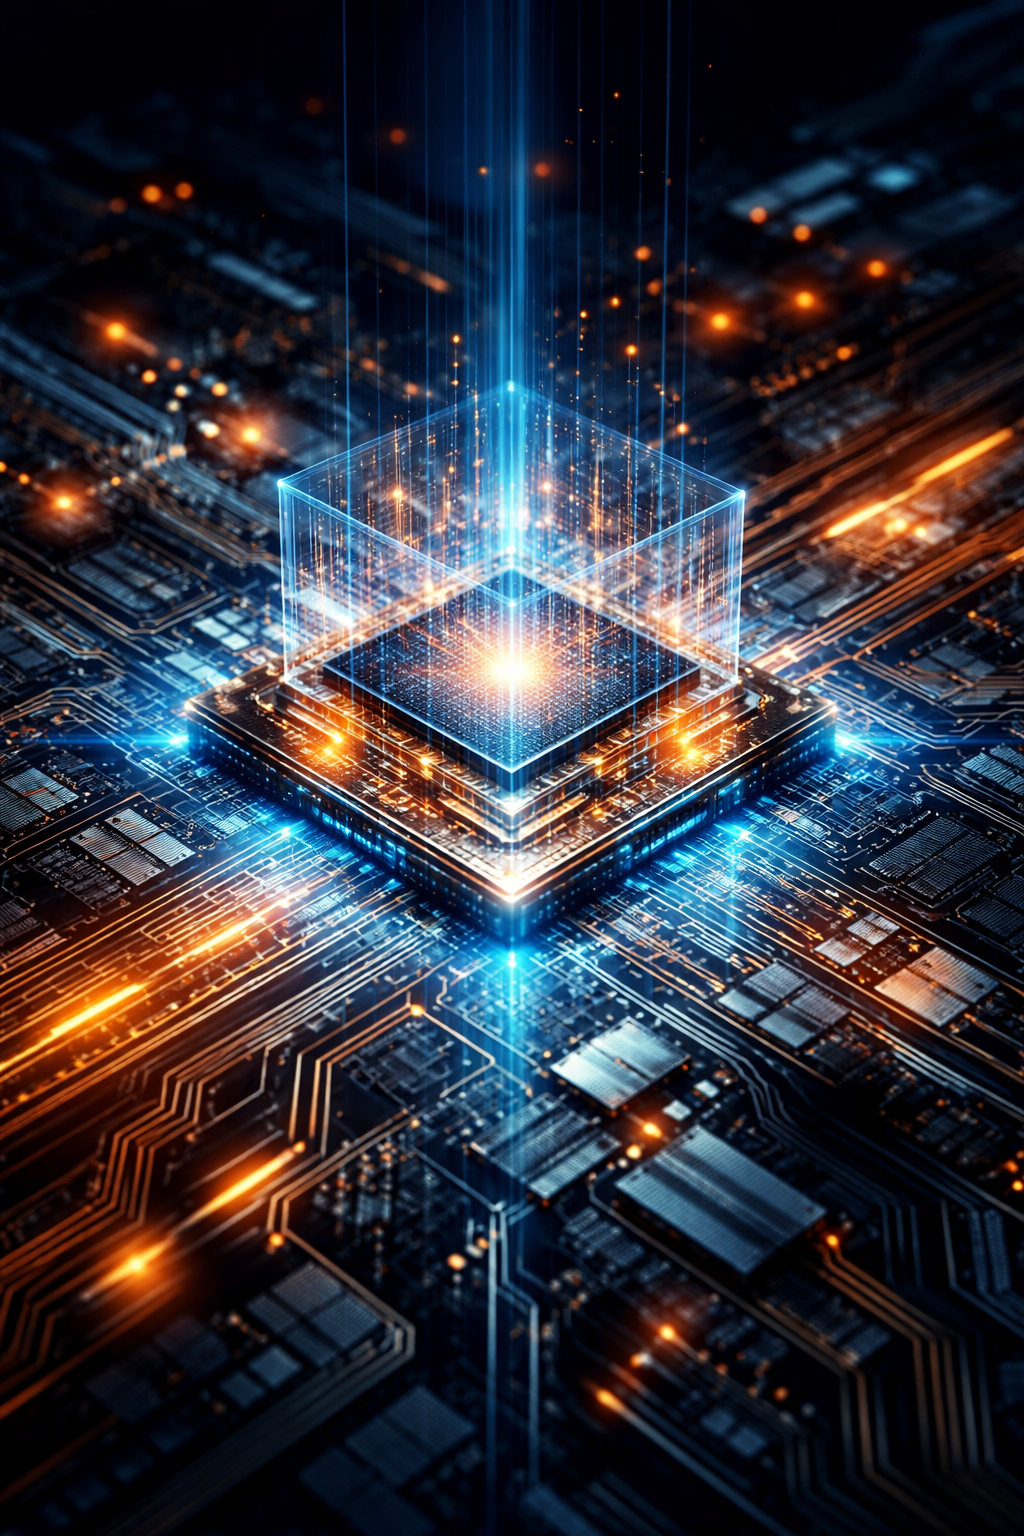
\includegraphics[width=\paperwidth]{gorseller/kapak-arkaplan.png}%
        };
    \end{scope}

    % === ALT BÖLGE: Koyu degrade (metin okunabilirliği için) ===
    % Alt %45: tamamen koyu
    \fill[pcbzemin, opacity=0.85]
        (current page.south west) rectangle ([yshift=13.5cm]current page.south east);
    % Kademeli geçiş bantları (yumuşak degrade etkisi)
    \fill[pcbzemin, opacity=0.7]
        ([yshift=13.5cm]current page.south west) rectangle ([yshift=14.5cm]current page.south east);
    \fill[pcbzemin, opacity=0.5]
        ([yshift=14.5cm]current page.south west) rectangle ([yshift=15.5cm]current page.south east);
    \fill[pcbzemin, opacity=0.3]
        ([yshift=15.5cm]current page.south west) rectangle ([yshift=16.5cm]current page.south east);
    \fill[pcbzemin, opacity=0.15]
        ([yshift=16.5cm]current page.south west) rectangle ([yshift=17.5cm]current page.south east);

    % === ÜST ŞERİT (ince altın çizgi) ===
    \fill[pcbaltin] (current page.north west) rectangle ([yshift=-1.2mm]current page.north east);

    % === ALT ŞERİT (ince altın çizgi) ===
    \fill[pcbaltin] ([yshift=1.2mm]current page.south west) rectangle (current page.south east);

    % === ANA BAŞLIK ===
    \node[font=\fontsize{42}{50}\selectfont\bfseries, text=pcbbeyaz]
        at ([yshift=9.5cm]current page.south) {Bilgisayar};
    \node[font=\fontsize{42}{50}\selectfont\bfseries, text=pcbbeyaz]
        at ([yshift=7.5cm]current page.south) {Mimarisi};

    % === ALTIN AYIRICI ÇİZGİ ===
    \draw[pcbaltin, line width=1.2pt]
        ([yshift=6.5cm, xshift=-3cm]current page.south) -- ++(6cm,0);

    % === ALT BAŞLIK ===
    \node[font=\Large\itshape, text=pcbacik]
        at ([yshift=5.5cm]current page.south) {RISC-V Tabanlı Yaklaşım};

    % === YAZAR ADI ===
    \node[font=\large\bfseries, text=pcbbeyaz]
        at ([yshift=3.8cm]current page.south) {Prof.\ Dr.\ Oğuz Ergin};

    % === BASKI BİLGİSİ ===
    \node[font=\normalsize, text=pcbaltin, opacity=0.7]
        at ([yshift=1.8cm]current page.south) {Sürüm 0.2.0\ \ $\cdot$\ \ \the\year};

\end{tikzpicture}
\vfill
\end{titlepage}


% Künye Sayfası (kapağın hemen arkası, sol sayfa)
\clearpage
\thispagestyle{empty}
\vspace*{\fill}
\noindent
{\small
\textbf{Bilgisayar Mimarisi} --- RISC-V Tabanlı Yaklaşım\\[3pt]
Prof.\ Dr.\ Oğuz Ergin\\[6pt]
Sürüm \kitapsurum, \the\year\\[6pt]
ISBN: 978-625-00-6081-0\\[12pt]
Bu kitap, lisans düzeyinde bilgisayar mimarisi derslerinde ders kitabı
olarak kullanılmak üzere hazırlanmıştır.\\[6pt]
Kitaptaki tüm mimari eser fotoğrafları Wikimedia Commons'tan
Creative Commons (CC BY-SA) lisansı altında alınmıştır.\\[6pt]
Tüm hakları saklıdır.
}
\vspace{2cm}

% İthaf
\cleardoublepage
\thispagestyle{empty}
\vspace*{\fill}
\begin{center}
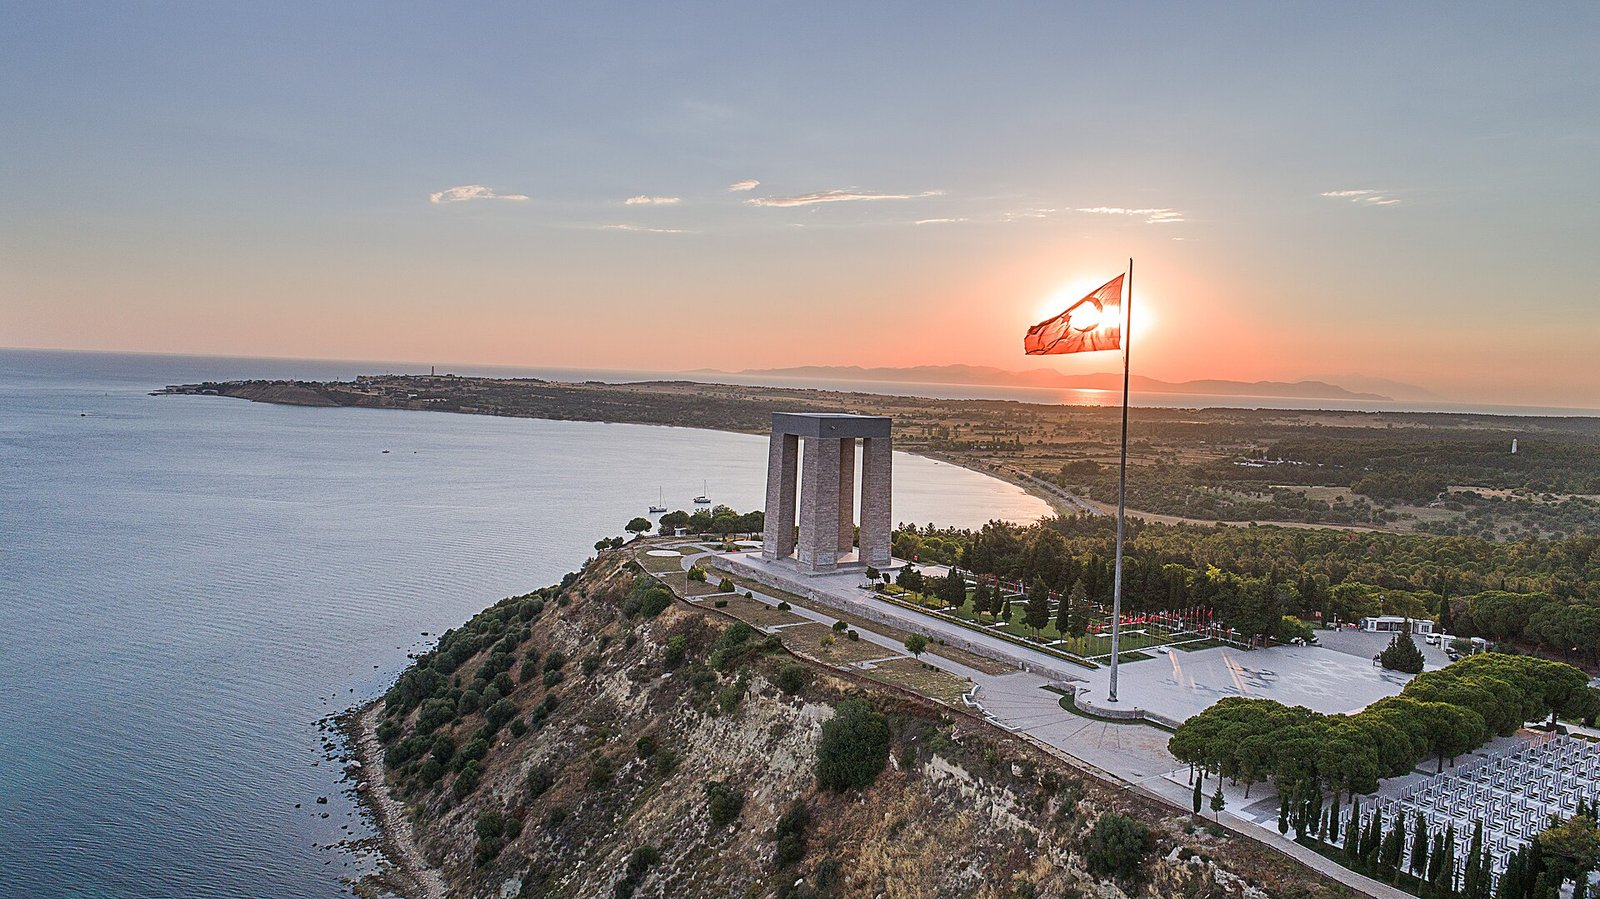
\includegraphics[width=0.95\textwidth]{gorseller/ithaf-canakkale.jpg}

\vspace{14pt}
\textit{\large Vatan uğruna can veren bu ülkenin\\[6pt]
gerçek mimarlarının anısına \ldots}
\end{center}
\vspace*{\fill}
\cleardoublepage

% Önsöz
\chapter*{Önsöz}
\addcontentsline{toc}{chapter}{Önsöz}

Bu kitap, lisans düzeyindeki bilgisayar mimarisi derslerinde kaynak kitap olarak kullanılmak üzere hazırlanmıştır. Kitabın amacı, bilgisayar mühendisliği ve ilgili mühendislik dallarındaki öğrencilere, çağdaş bilgisayar sistemlerinin temel yapısını ve çalışma prensiplerini Türkçe olarak sunmaktır.

Kitap boyunca RISC-V buyruk kümesi mimarisi temel alınmıştır. RISC-V, açık kaynaklı ve modüler yapısıyla hem akademik hem de endüstriyel alanda giderek yaygınlaşan çağdaş bir mimaridir. Bu tercih, öğrencilerin güncel ve geleceğe yönelik bir mimari üzerinden kavramları öğrenmesini sağlamaktadır.

İlk bölümde bilgisayarların tarihsel gelişimi ve temel kavramlar ele alınmaktadır. İkinci bölümde başarım değerlendirmesi, üçüncü bölümde buyruk kümesi mimarisi, dördüncü bölümde RISC-V ile programlama, beşinci bölümde aritmetik işlemler, altıncı bölümde işlemci tasarımı ve yedinci bölümde boru hattı yöntemleri anlatılmaktadır. Sekizinci bölüm bellek hiyerarşisine, dokuzuncu bölüm giriş/çıkış sistemlerine ayrılmıştır. Onuncu bölümde çok çekirdekli işlemciler, on birinci bölümde GPU ve hızlandırıcılar, on ikinci bölümde ise güncel mimari eğilimleri tartışılmaktadır. Ek~A'da sayı sistemleri ve kodlama, Ek~B'de sayısal tasarım temelleri, Ek~C'de RISC-V referans kartı, Ek~D'de ise uygulamalı çalışma rehberi ve mini projeler sunulmaktadır.

Türkiye'de bilgisayar mimarisi alanında Türkçe kaynak üretme çabası uzun bir geçmişe sahiptir. Eşref Adalı'nın \emph{Mikroişlemciler Mikrobilgisayarlar}~\cite{adali} kitabı, M.~Morris Mano'nun Türkçeye çevrilen \emph{Bilgisayar Sistemleri Mimarisi}~\cite{mano2002tr} eseri, Mehmet Bodur'un EMO yayını olan \emph{Bilgisayar Organizasyonu: RISC Donanımına Giriş}~\cite{bodur2003} kitabı, Şirzat Kahramanlı'nın \emph{Bilgisayar Mimarisi}~\cite{kahramanli} eseri, Patterson ve Hennessy'nin Türkçeye kazandırılan \emph{Bilgisayar Mimarisi ve Tasarım}~\cite{patterson2021tr} çevirisi ve Cengiz Uğurkaya ile Osman Aliefendioğlu'nun \emph{Çağdaş Bilgisayar Mimarisi}~\cite{colkesen2026} kitabı bu alandaki öncü çalışmalardır. Bu kitap, söz konusu değerli çabaların bir sonraki adımı olarak RISC-V buyruk kümesi mimarisi üzerine odaklanmakta ve açık erişim felsefesiyle Türkçe teknik içerik birikimine katkı sunmayı amaçlamaktadır.

Her bölümün başında, Türkiye'nin mimari mirasından bir eser fotoğrafı yer almaktadır. Bu eserler, bilgisayar mimarisi kavramlarıyla tematik bir bağ kurularak seçilmiştir.

Bu kitabın hazırlanmasında destek ve katkılarından dolayı Kasırga araştırma takımındaki öğrencilerime teşekkür ederim.

\vspace{1cm}
\begin{flushright}
\textit{Oğuz Ergin}\\
Ankara, \the\year
\end{flushright}
\cleardoublepage

% İçindekiler
\tableofcontents
\cleardoublepage
\listoffigures
\addcontentsline{toc}{chapter}{Şekil Listesi}
\cleardoublepage
\listoftables
\addcontentsline{toc}{chapter}{Tablo Listesi}
\cleardoublepage
\listofbilginotlari

% --- Ana İçerik ---
\mainmatter

\bolumekle{bolum01-giris/bolum01}{chap:giris}{1}{Bilgisayar Mimarisine Giriş}
\bolumekle{bolum02-basarim/bolum02}{chap:basarim}{2}{Bilgisayar Başarımı}
\bolumekle{bolum03-buyruk-kumesi/bolum03}{chap:buyruk-kumesi}{3}{Buyruk Kümesi Mimarisi}
\bolumekle{bolum04-programlama/bolum04-programlama}{chap:programlama}{4}{RISC-V ile Programlama}
\bolumekle{bolum05-aritmetik/bolum05}{chap:aritmetik}{5}{Aritmetik İşlemler}
\bolumekle{bolum06-islemci-tasarimi/bolum06}{chap:islemci-tasarimi}{6}{İşlemci Tasarımı}
\bolumekle{bolum07-boru-hatti/bolum07}{chap:boruhatti}{7}{Boru Hattı}
\bolumekle{bolum08-bellek/bolum08}{chap:bellek}{8}{Bellek}
\bolumekle{bolum09-giris-cikis/bolum09}{chap:giris-cikis}{9}{Giriş ve Çıkış Aygıtları}
\bolumekle{bolum10-cok-cekirdekli/bolum10}{chap:cok-cekirdekli}{10}{Çok Çekirdekli ve Koşut İşlemciler}
\bolumekle{bolum11-gpu-hizlandiricilar/bolum11}{chap:gpu-hizlandiricilar}{11}{GPU ve Hızlandırıcılar}
\bolumekle{bolum12-guncel-mimariler/bolum12}{chap:guncel-mimariler}{12}{Güncel Mimari Eğilimleri}

% --- Ekler ---
\appendix
\ekekle{ekA-sayi-sistemleri/ekA}{ch:sayi-sistemleri}{A}{Sayı Sistemleri ve Kodlama}
\ekekle{ekB-sayisal-tasarim/ekB}{ch:sayisal-tasarim}{B}{Sayısal Tasarım Temelleri}
\ekekle{ekC-risc-v-referans/ekC}{app:risc-v-referans}{C}{RISC-V Referans Kartı}
\ekekle{ekD-pratik-rehber/ekD}{app:pratik-rehber}{D}{RISC-V Uygulama Çalışmaları ve Projeler}

% --- Arka Sayfalar ---
\backmatter

% Terimler Sözlüğü
\chapter*{Terimler Sözlüğü}
\addcontentsline{toc}{chapter}{Terimler Sözlüğü}
% =============================================================
% Terimler Sözlüğü -- Türkçe-İngilizce / İngilizce-Türkçe
% Bilgisayar Mimarisi Kitabı
% Bu dosya % =============================================================
% Terimler Sözlüğü -- Türkçe-İngilizce / İngilizce-Türkçe
% Bilgisayar Mimarisi Kitabı
% Bu dosya % =============================================================
% Terimler Sözlüğü -- Türkçe-İngilizce / İngilizce-Türkçe
% Bilgisayar Mimarisi Kitabı
% Bu dosya \input{terimler-sozlugu} ile dahil edilir.
% \chapter komutu ana-kitap.tex dosyasında tanımlanmalıdır.
% =============================================================

%% ============================================================
%%  BÖLÜM 1: Türkçe → İngilizce
%%  Türkçe alfabetik sıra: a,b,c,ç,d,e,f,g,ğ,h,ı,i,j,k,l,m,
%%                          n,o,ö,p,r,s,ş,t,u,ü,v,y,z
%% ============================================================
\section*{Türkçe -- İngilizce}
\addcontentsline{toc}{section}{Türkçe -- İngilizce}

{\small
\begin{longtable}{@{}p{7.6cm}p{7.6cm}@{}}
\toprule
\textbf{Türkçe Terim} & \textbf{İngilizce Karşılık} \\
\midrule
\endfirsthead

\toprule
\textbf{Türkçe Terim (devam)} & \textbf{İngilizce Karşılık} \\
\midrule
\endhead

\midrule
\multicolumn{2}{r}{\small\textit{(devamı sonraki sayfada)}} \\
\endfoot

\bottomrule
\endlastfoot

%% --- A ---
adresleme kipleri & addressing modes \\
ağırlıklı ortalama & weighted average \\
Akış Çoklu İşlemci (\texttt{SM}) & Streaming Multiprocessor (\texttt{SM}) \\
altyordam & subroutine \\
Amdahl Yasası & Amdahl's Law \\
\texttt{AMB} & \texttt{ALU} (Arithmetic Logic Unit) \\
anlamlı kısım & significand / mantissa \\
anlık değer & immediate value \\
anlık değer üreteci & immediate generator \\
ara bellek & buffer \\
ardışık tutarlılık & sequential consistency \\
arama zamanı & seek time \\
aritmetik buyruklar & arithmetic instructions \\
aşınma dengeleme & wear leveling \\
aritmetik mantık birimi (\texttt{AMB}) & Arithmetic Logic Unit (\texttt{ALU}) \\
aritmetik yoğunluk & arithmetic intensity \\
artık-N gösterimi & excess-N notation \\
\texttt{ASCII} & \texttt{ASCII} \\
\texttt{ASIC} & Application-Specific Integrated Circuit \\
çevirici dil (Assembly) & assembly language \\
atlama buyrukları & jump instructions \\
atomik işlem & atomic operation \\
aygıt & device \\
ayrıcalıklı kip & privileged mode \\

%% --- B ---
bilimsel gösterim & scientific notation \\
Booth algoritması & Booth's algorithm \\
B türü & B-type \\
bağlam değiştirme & context switching \\
bağlantı noktası & port \\
bağlayıcı & linker \\
bakış tablosu (\texttt{LUT}) & Look-Up Table (\texttt{LUT}) \\
bant genişliği & bandwidth \\
başarım & performance \\
bayat veri & stale data \\
bayt & byte \\
bayt sıralaması & byte order \\
büyük sayfa & huge page \\
\texttt{BBÇ} & \texttt{CPI} (cycles per instruction) \\
\texttt{BCD} & Binary-Coded Decimal \\
bellek & memory \\
bellek birleştirme & memory coalescing \\
bellek denetleyicisi & memory controller \\
bellek duvarı & memory wall \\
bellek koruması & memory protection \\
bellek hizalama & memory alignment \\
bellek hiyerarşisi & memory hierarchy \\
bellek tutarlığı & cache coherence \\
bellek tutarlık modeli & memory consistency model \\
bellekle eşlemeli G/Ç & memory-mapped I/O \\
benchmark & sınama programı (denektaşı) \\
big.LITTLE & big.LITTLE \\
bire tümleyen & one's complement \\
birleşik bellek mimarisi & unified memory architecture \\
birleşik devre & combinational circuit \\
bit & bit \\
blok & block \\
boru hattı & pipeline \\
boru hattı aşaması & pipeline stage \\
boru hattı kaydı & pipeline register \\
boru hattı tehlikesi & pipeline hazard \\
boşluk (boru hattı) & bubble / NOP \\
bölme & division \\
bulamama (önbellekte) & miss (cache miss) \\
bulamama cezası & miss penalty \\
bulamama oranı & miss rate \\
bulma (önbellekte) & hit (cache hit) \\
bulma oranı & hit rate \\
buyruk & instruction \\
buyruk başına çevrim (\texttt{BBÇ}) & cycles per instruction (\texttt{CPI}) \\
buyruk belleği & instruction memory \\
buyruk çözme & instruction decode \\
buyruk düzeyi paralelliği & instruction-level parallelism (\texttt{ILP}) \\
buyruk biçimi & instruction format \\
buyruk getirme birimi & instruction fetch unit \\
buyruk kümesi mimarisi & Instruction Set Architecture (\texttt{ISA}) \\
buyruk önbelleği & instruction cache \\
buyruk sayacı & instruction counter \\
büyüğü başta & big-endian \\

%% --- C ---
chiplet & chiplet \\
\texttt{CISC} & Complex Instruction Set Computer \\
\texttt{CMOS} & Complementary \texttt{MOS} \\
\texttt{CUDA} & Compute Unified Device Architecture \\

%% --- Ç ---
\texttt{ÇBB} & \texttt{IPC} (instructions per cycle) \\
çağrı kuralları & calling conventions \\
çarpma & multiplication \\
çarpma-toplama (\texttt{MAC}) & multiply-accumulate (\texttt{MAC}) \\
çatı çizgisi modeli & roofline model \\
çekirdek & core \\
çekirdek fonksiyonu (GPU) & kernel function \\
çerçeve göstergesi & frame pointer \\
çevirici & assembler \\
çevrim & cycle \\
çevrim başına buyruk (\texttt{ÇBB}) & instructions per cycle (\texttt{IPC}) \\
çevrim zamanı & cycle time \\
çıkarım (yapay zeka) & inference \\
çıkarma & subtraction \\
yonga içi bağlantı ağı (\texttt{NoC}) & Network on Chip (\texttt{NoC}) \\
çok çekirdekli işlemci & multi-core processor \\
çok seviyeli sayfa tablosu & multi-level page table \\
çok çevrimli & multi-cycle \\
çok vuruşluk işlemci & multi-cycle processor \\
çoklayıcı & multiplexer \\
çözgü & warp \\
çözgü sapması & warp divergence \\

%% --- D ---
dağıtık bellek & distributed memory \\
durum yazmacı & state register \\
dalga eldeli toplayıcı & ripple carry adder \\
dallanma buyrukları & branch instructions \\
dallanma hedef ara belleği & branch target buffer (BTB) \\
dallanma öngörüsü & branch prediction \\
darboğaz & bottleneck \\
\texttt{DDR} & Double Data Rate \\
DEĞİL kapısı & \texttt{NOT} gate \\
dekoder & decoder \\
denetim birimi & control unit \\
denetim sinyali & control signal \\
denetim tablosu & control table \\
denetim tehlikesi & control hazard \\
devingen güç tüketimi & dynamic power consumption \\
devingen öngörü & dynamic prediction \\
Dennard ölçeklemesi & Dennard scaling \\
derin öğrenme & deep learning \\
derleyici & compiler \\
dikey mikroprogramlama & vertical microprogramming \\
dizin tabanlı protokol & directory-based protocol \\
\texttt{DMA} & Direct Memory Access \\
\texttt{DRAM} & Dynamic Random Access Memory \\
doğrudan eşlemeli önbellek & direct-mapped cache \\
doğruluk tablosu & truth table \\
dönme gecikmesi & rotational latency \\
doğrudan yazma & write-through \\
doku belleği & texture memory \\
dolanıklık & entanglement \\
doluluk & occupancy \\
donanım & hardware \\
donanımsal çok kanallılık & hardware multithreading \\
dönüş adresi & return address \\
döngüsel kilit & spin-lock \\
durağan öngörü & static prediction \\
durağan güç tüketimi & static power consumption (leakage) \\
durma & stall \\
düzenleme birimi & hazard detection unit \\

%% --- E ---
\texttt{EDVAC} & \texttt{EDVAC} \\
eğitim (yapay zeka) & training \\
elde & carry \\
elden önceden üretme & carry lookahead \\
\texttt{ENIAC} & \texttt{ENIAC} \\
engel & barrier \\
eşlik (RAID) & parity (RAID) \\
erişim süresi & access time \\
eşzamanlama & synchronization \\
eşzamanlı çok kanallılık (\texttt{SMT}) & Simultaneous Multithreading (\texttt{SMT}) \\
eşzamanlılık & concurrency \\
etiket & tag \\
etkin adres & effective address \\

%% --- F ---
Flaş çeviri katmanı (\texttt{FTL}) & Flash Translation Layer (\texttt{FTL}) \\
flaş bellek & flash memory \\
flip-flop & flip-flop \\
\texttt{FPGA} & Field-Programmable Gate Array \\

%% --- G ---
gecikme & latency \\
geometrik ortalama & geometric mean \\
gecikme odaklı tasarım & latency-oriented design \\
geciktirilmiş dallanma & delayed branching \\
gerçek veri bağımlılığı & true data dependence \\
genel amaçlı yazmaç & general-purpose register \\
genel bellek & global memory \\
geri yazma & write-back \\
getir-çöz-yürüt döngüsü & fetch-decode-execute cycle \\
gevşek tutarlılık & relaxed consistency \\
giriş/çıkış (\texttt{G/Ç}) & input/output (\texttt{I/O}) \\
gölgelendirici & shader \\
gözetleme protokolü & snooping protocol \\
\texttt{GPGPU} & General-Purpose computing on GPU \\
\texttt{GPU} & Graphics Processing Unit \\
gshare öngörücü & gshare predictor \\
Gustafson Yasası & Gustafson's Law \\
güç duvarı & power wall \\
güç tüketimi & power consumption \\

%% --- Ğ ---

%% --- H ---
Harvard mimarisi & Harvard architecture \\
\texttt{HBM} & High Bandwidth Memory \\
heterojen hesaplama & heterogeneous computing \\

%% --- Önbellekte bulamama terimleri (B harfi altında da var) ---
%% --- I ---
ızgara & grid \\

%% --- İ ---
I türü & I-type \\
\texttt{IEEE 754} & \texttt{IEEE 754} \\
yol & bus \\
ikincil bellek & secondary storage \\
\texttt{IOPS} & Input/Output Operations Per Second \\
ikiye tümleyen & two's complement \\
ikilik taban & binary \\
%% isabet → bulma olarak B harfi altında (bkz. "bulma")
iş çıkarma oranı & throughput \\
iş parçacığı & thread \\
iş parçacığı düzeyi paralelliği & thread-level parallelism \\
iş parçacığı havuzu & thread pool \\
işaret biti & sign bit \\
işaretli genişletme & sign extension \\
işaretli & signed \\
işaretsiz & unsigned \\
işlem kodu & opcode \\
işlemci & processor \\
işletim sistemi & operating system \\
istisna (boru hattı) & exception (pipeline) \\

%% --- J ---
J türü & J-type \\

%% --- K ---
kritik yol & critical path \\
karşı bağımlılık & anti-dependence \\
karşılaştırma buyrukları & comparison instructions \\
kaydırma buyrukları & shift instructions \\
kayan nokta & floating point \\
kayan noktalı sayı birimi & floating point unit (\texttt{FPU}) \\
katı hal sürücü (\texttt{SSD}) & Solid State Drive (\texttt{SSD}) \\
kesin istisna & precise exception \\
kesme & interrupt \\
kesme denetleyicisi & interrupt controller \\
kesme hizmet yordamı & interrupt service routine \\
kilit & lock/mutex \\
kilitlenme & deadlock \\
kod çözücü & decoder \\
koşullu dallanma & conditional branch \\
koşulsuz dallanma & unconditional branch \\
kuantum hesaplama & quantum computing \\
kübit & qubit \\
küçüğü başta & little-endian \\
kırmık & die \\
küme ilişkili & set associative \\

%% --- L ---
L1 önbellek & L1 cache \\
L2 önbellek & L2 cache \\
L3 önbellek & L3 cache \\

%% --- M ---
\texttt{M.2} & \texttt{M.2} (form factor) \\
makine dili & machine language \\
makro buyruk & macro instruction \\
\texttt{MLC} & Multi-Level Cell \\
mantık buyrukları & logic instructions \\
mantık kapısı & logic gate \\
matris çarpımı & matrix multiplication \\
Meltdown & Meltdown \\
\texttt{MESI} protokolü & \texttt{MESI} protocol \\
merkezi işlem birimi (\texttt{MİB}) & Central Processing Unit (\texttt{CPU}) \\
mesaj geçirme & message passing \\
\texttt{MFLOPS} & Millions of Floating Point Operations Per Second \\
mikro buyruk & micro-operation \\
mikro program belleği & control store \\
mikromimari & microarchitecture \\
mikroprogramlama & microprogramming \\
\texttt{MIPS} & Millions of Instructions Per Second \\
\texttt{MİB} & \texttt{CPU} (Central Processing Unit) \\
Moore Yasası & Moore's Law \\

%% --- N ---
\texttt{NAND} Flaş bellek & \texttt{NAND Flash} memory \\
\texttt{NUMA} & Non-Uniform Memory Access \\
\texttt{NVMe} & Non-Volatile Memory Express \\

%% --- O ---
olağanlaştırma & normalization \\
on altılık taban & hexadecimal \\
optimal çıkarma algoritması & optimal (Bélády's) replacement algorithm \\
ortalama bellek erişim süresi (\texttt{AMAT}) & Average Memory Access Time (\texttt{AMAT}) \\

%% --- Ö ---
önbellek & cache \\
önbellek satırı & cache line \\
önceden getirme & prefetching \\
Özel VEYA kapısı & \texttt{XOR} gate \\
özel fonksiyon birimi (\texttt{SFU}) & Special Function Unit (\texttt{SFU}) \\

%% --- P ---
paralel hesaplama & parallel computing \\
paralel verimlilik & parallel efficiency \\
paylaşımlı bellek & shared memory \\
\texttt{PCI} Express & \texttt{PCI} Express \\
program sayacı & program counter \\

%% --- Q ---
\texttt{QLC} & Quad-Level Cell \\

%% --- R ---
R türü & R-type \\
\texttt{RAID} & Redundant Array of Independent Disks \\
\texttt{RISC} & Reduced Instruction Set Computer \\
\texttt{RISC-V} & \texttt{RISC-V} \\

%% --- S ---
S türü & S-type \\
sıfırla genişletme & zero extension \\
saat çevrimi & clock cycle \\
saat sıklığı & clock frequency \\
sabit bellek & constant memory \\
sabit disk sürücüsü (\texttt{HDD}) & hard disk drive (\texttt{HDD}) \\
\texttt{SATA} & Serial \texttt{ATA} \\
saklama buyruğu & store instruction \\
sanal adres & virtual address \\
sanal bellek & virtual memory \\
sayfa & page \\
sayfa hatası & page fault \\
sayfa tablosu & page table \\
sekizlik taban & octal \\
semafor & semaphore \\
sıra dışı yürütme & out-of-order execution \\
şeritleme & striping \\
\texttt{SIMD} & Single Instruction, Multiple Data \\
\texttt{SLC} & Single-Level Cell \\
\texttt{SIMT} & Single Instruction, Multiple Threads \\
Sinir Ağı İşlem Birimi (\texttt{NPU}) & Neural Processing Unit (\texttt{NPU}) \\
sınama programı (denektaşı) & benchmark \\
sistolik dizi & systolic array \\
Soğutma Tasarım Gücü (\texttt{TDP}) & Thermal Design Power (\texttt{TDP}) \\
\texttt{SoC} & System on Chip \\
sonlu durum makinesi & finite state machine \\
sonuç bağımlılığı & output dependence \\
sonradan yazma & write-back \\
soyutlama & abstraction \\
sözde buyruk & pseudo-instruction \\
sözde-EUZK & pseudo-LRU \\
Spectre & Spectre \\
\texttt{SPEC} & \texttt{SPEC} \\
spekülatif yürütme & speculative execution \\
\texttt{SRAM} & Static Random Access Memory \\
Sv39 (RISC-V) & Sv39 (39-bit virtual addressing) \\
Sv48 (RISC-V) & Sv48 (48-bit virtual addressing) \\
Sv57 (RISC-V) & Sv57 (57-bit virtual addressing) \\
çoklu buyruk başlatımlı & superscalar \\
süperpozisyon & superposition \\

%% --- Ş ---

%% --- T ---
tam ilişkili & fully associative \\
Thunderbolt & Thunderbolt \\
\texttt{TLC} & Triple-Level Cell \\
\texttt{TRIM} & \texttt{TRIM} \\
tam sayı & integer \\
tam toplayıcı & full adder \\
taşma & overflow \\
tek çevrimli & single-cycle \\
tek vuruşluk işlemci & single-cycle processor \\
tekdüze bellek erişimi & Uniform Memory Access (\texttt{UMA}) \\
tekdüze olmayan bellek erişimi & Non-Uniform Memory Access (\texttt{NUMA}) \\
Tensör çekirdeği & Tensor Core \\
Tensör İşlem Birimi (\texttt{TPU}) & Tensor Processing Unit (\texttt{TPU}) \\
\texttt{TLB} & Translation Lookaside Buffer \\
toplama & addition \\
transistör & transistor \\
turnuva öngörücüsü & tournament predictor \\
tümleşik devre & integrated circuit \\

%% --- U ---
uç bilgi işlem & edge computing \\
U türü & U-type \\
\texttt{USB} & Universal Serial Bus \\
\texttt{UCIe} & Universal Chiplet Interconnect Express \\
\texttt{UMA} & Uniform Memory Access \\
Unicode & Unicode \\
uzamsal yerellik & spatial locality \\

%% --- Ü ---
üç C modeli (3C modeli) & three Cs model \\
üs & exponent \\
üst anlık buyruklar & upper immediate instructions \\

%% --- V ---
vakum tüpü & vacuum tube \\
VE kapısı & \texttt{AND} gate \\
veri akış mimarisi & dataflow architecture \\
veri aktarma buyrukları & data transfer instructions \\
veri bağımlılığı & data dependency \\
veri belleği & data memory \\
veri tehlikesi & data hazard \\
veri yolu & datapath \\
veri yönlendirmesi & forwarding \\
verim & throughput \\
verim odaklı tasarım & throughput-oriented design \\
Verilog & Verilog \\
VEYA kapısı & \texttt{OR} gate \\
\texttt{VHDL} & \texttt{VHDL} \\
\texttt{VLSI} & Very Large-Scale Integration \\
Von Neumann darboğazı & Von Neumann bottleneck \\
Von Neumann mimarisi & Von Neumann architecture \\

%% --- Y ---
yan kanal saldırısı & side-channel attack \\
yanlış paylaşım & false sharing \\
yapay sınama programları & synthetic benchmarks \\
yapay zeka & artificial intelligence \\
yapısal tehlike & structural hazard \\
yarım toplayıcı & half adder \\
yarış durumu & race condition \\
yatay mikroprogramlama & horizontal microprogramming \\
yazılım & software \\
yazma geçersizleştirme & write-invalidate \\
yazma güncelleme & write-update \\
yazma serileştirmesi & write serialization \\
yazma tahsisli & write-allocate \\
yazma tahsissiz & no-write-allocate \\
yazma ara belleği & write buffer \\
yazma yayılımı & write propagation \\
yazmaç & register \\
yazmaç aktarım düzeyi (\texttt{RTL}) & Register Transfer Level (\texttt{RTL}) \\
yazmaç öbeği & register file \\
yazmaç yeniden adlandırma & register renaming \\
yekpare kırmık & monolithic die \\
yeniden yapılandırılabilir hesaplama & reconfigurable computing \\
yerel bellek & local memory \\
yerellik ilkesi & locality principle \\
yığıt & stack \\
yığıt göstergesi & stack pointer \\
yonga & chip \\
yuvarlama & rounding \\
yükleyici & loader \\
yükle-kullan sorunu & load-use hazard \\
yükleme buyruğu & load instruction \\
yürütme birimi & execution unit \\
yürütme zamanı & execution time \\

%% --- Z ---
zamansal yerellik & temporal locality \\

\end{longtable}
}


\bigskip

%% ============================================================
%%  BÖLÜM 2: İngilizce → Türkçe
%%  İngilizce alfabetik sıra (A-Z)
%% ============================================================
\section*{İngilizce -- Türkçe}
\addcontentsline{toc}{section}{İngilizce -- Türkçe}

{\small
\begin{longtable}{@{}p{7.6cm}p{7.6cm}@{}}
\toprule
\textbf{İngilizce Terim} & \textbf{Türkçe Karşılık} \\
\midrule
\endfirsthead

\toprule
\textbf{İngilizce Terim (cont.)} & \textbf{Türkçe Karşılık} \\
\midrule
\endhead

\midrule
\multicolumn{2}{r}{\small\textit{(continued on next page)}} \\
\endfoot

\bottomrule
\endlastfoot

%% --- A ---
abstraction & soyutlama \\
access time & erişim süresi \\
addition & toplama \\
Average Memory Access Time (\texttt{AMAT}) & ortalama bellek erişim süresi (\texttt{AMAT}) \\
addressing modes & adresleme kipleri \\
Amdahl's Law & Amdahl Yasası \\
\texttt{AND} gate & VE kapısı \\
anti-dependence & karşı bağımlılık \\
Application-Specific Integrated Circuit (\texttt{ASIC}) & \texttt{ASIC} \\
Arithmetic Logic Unit (\texttt{ALU}) & aritmetik mantık birimi (\texttt{AMB}) \\
arithmetic instructions & aritmetik buyruklar \\
arithmetic intensity & aritmetik yoğunluk \\
artificial intelligence & yapay zeka \\
\texttt{ASCII} & \texttt{ASCII} \\
assembler & çevirici \\
assembly language & çevirici dil \\
atomic operation & atomik işlem \\

%% --- B ---
B-type & B türü \\
Booth's algorithm & Booth algoritması \\
bandwidth & bant genişliği \\
barrier & engel \\
benchmark & sınama programı (denektaşı) \\
big-endian & büyüğü başta \\
big.LITTLE & big.LITTLE \\
binary & ikilik taban \\
Binary-Coded Decimal (\texttt{BCD}) & \texttt{BCD} \\
bit & bit \\
block & blok \\
bottleneck & darboğaz \\
branch instructions & dallanma buyrukları \\
branch prediction & dallanma öngörüsü \\
branch target buffer (BTB) & dallanma hedef ara belleği \\
buffer & ara bellek \\
bubble (pipeline) & boşluk (boru hattı) \\
bus & yol \\
byte & bayt \\
byte order & bayt sıralaması \\

%% --- C ---
cache & önbellek \\
cache coherence & bellek tutarlığı \\
cache line & önbellek satırı \\
calling conventions & çağrı kuralları \\
carry & elde \\
carry lookahead & elden önceden üretme \\
Central Processing Unit (\texttt{CPU}) & merkezi işlem birimi (\texttt{MİB}) \\
chip & yonga \\
chiplet & chiplet \\
clock cycle & saat çevrimi \\
clock frequency & saat sıklığı \\
combinational circuit & birleşik devre \\
Complementary \texttt{MOS} (\texttt{CMOS}) & \texttt{CMOS} \\
compiler & derleyici \\
comparison instructions & karşılaştırma buyrukları \\
Complex Instruction Set Computer (\texttt{CISC}) & \texttt{CISC} \\
Compute Unified Device Architecture (\texttt{CUDA}) & \texttt{CUDA} \\
concurrency & eşzamanlılık \\
conditional branch & koşullu dallanma \\
constant memory & sabit bellek \\
context switching & bağlam değiştirme \\
control hazard & denetim tehlikesi \\
control signal & denetim sinyali \\
control store & mikro program belleği \\
control table & denetim tablosu \\
control unit & denetim birimi \\
core & çekirdek \\
critical path & kritik yol \\
cycle & çevrim \\
cycle time & çevrim zamanı \\
cycles per instruction (\texttt{CPI}) & buyruk başına çevrim (\texttt{BBÇ}) \\

%% --- D ---
die & kırmık \\
data dependency & veri bağımlılığı \\
data hazard & veri tehlikesi \\
data memory & veri belleği \\
data transfer instructions & veri aktarma buyrukları \\
dataflow architecture & veri akış mimarisi \\
datapath & veri yolu \\
deadlock & kilitlenme \\
decoder & dekoder / kod çözücü \\
deep learning & derin öğrenme \\
delayed branching & geciktirilmiş dallanma \\
Dennard scaling & Dennard ölçeklemesi \\
device & aygıt \\
Direct Memory Access (\texttt{DMA}) & \texttt{DMA} \\
direct-mapped cache & doğrudan eşlemeli önbellek \\
directory-based protocol & dizin tabanlı protokol \\
distributed memory & dağıtık bellek \\
division & bölme \\
Double Data Rate (\texttt{DDR}) & \texttt{DDR} \\
dynamic prediction & devingen öngörü \\
dynamic power consumption & devingen güç tüketimi \\
Dynamic Random Access Memory (\texttt{DRAM}) & \texttt{DRAM} \\

%% --- E ---
edge computing & uç bilgi işlem \\
\texttt{EDVAC} & \texttt{EDVAC} \\
effective address & etkin adres \\
\texttt{ENIAC} & \texttt{ENIAC} \\
entanglement & dolanıklık \\
exception (pipeline) & istisna (boru hattı) \\
excess-N notation & artık-N gösterimi \\
execution time & yürütme zamanı \\
execution unit & yürütme birimi \\
exponent & üs \\

%% --- F ---
false sharing & yanlış paylaşım \\
fetch-decode-execute cycle & getir-çöz-yürüt döngüsü \\
Field-Programmable Gate Array (\texttt{FPGA}) & \texttt{FPGA} \\
finite state machine & sonlu durum makinesi \\
flash memory & flaş bellek \\
Flash Translation Layer (\texttt{FTL}) & Flaş çeviri katmanı (\texttt{FTL}) \\
flip-flop & flip-flop \\
floating point & kayan nokta \\
floating point unit (\texttt{FPU}) & kayan noktalı sayı birimi \\
forwarding & veri yönlendirmesi \\
frame pointer & çerçeve göstergesi \\
full adder & tam toplayıcı \\
fully associative & tam ilişkili \\

%% --- G ---
General-Purpose computing on GPU (\texttt{GPGPU}) & \texttt{GPGPU} \\
general-purpose register & genel amaçlı yazmaç \\
geometric mean & geometrik ortalama \\
global memory & genel bellek \\
Graphics Processing Unit (\texttt{GPU}) & \texttt{GPU} \\
grid & ızgara \\
gshare predictor & gshare öngörücü \\
Gustafson's Law & Gustafson Yasası \\

%% --- H ---
half adder & yarım toplayıcı \\
hard disk drive (\texttt{HDD}) & sabit disk sürücüsü \\
hardware & donanım \\
hardware multithreading & donanımsal çok kanallılık \\
Harvard architecture & Harvard mimarisi \\
hazard detection unit & düzenleme birimi \\
heterogeneous computing & heterojen hesaplama \\
hexadecimal & on altılık taban \\
High Bandwidth Memory (\texttt{HBM}) & \texttt{HBM} \\
hit (cache hit) & bulma (önbellekte) \\
hit rate & bulma oranı \\
horizontal microprogramming & yatay mikroprogramlama \\
huge page & büyük sayfa \\

%% --- I ---
I-type & I türü \\
\texttt{IEEE 754} & \texttt{IEEE 754} \\
immediate generator & anlık değer üreteci \\
immediate value & anlık değer \\
inference (AI) & çıkarım (yapay zeka) \\
Input/Output Operations Per Second (\texttt{IOPS}) & \texttt{IOPS} \\
input/output (\texttt{I/O}) & giriş/çıkış (\texttt{G/Ç}) \\
instruction & buyruk \\
instruction cache & buyruk önbelleği \\
instruction decode & buyruk çözme \\
instruction counter & buyruk sayacı \\
instruction fetch unit & buyruk getirme birimi \\
instruction format & buyruk biçimi \\
instruction memory & buyruk belleği \\
Instruction Set Architecture (\texttt{ISA}) & buyruk kümesi mimarisi \\
instruction-level parallelism (\texttt{ILP}) & buyruk düzeyi paralelliği \\
instructions per cycle (\texttt{IPC}) & çevrim başına buyruk (\texttt{ÇBB}) \\
integer & tam sayı \\
integrated circuit & tümleşik devre \\
interrupt & kesme \\
interrupt controller & kesme denetleyicisi \\
interrupt service routine & kesme hizmet yordamı \\

%% --- J ---
J-type & J türü \\
jump instructions & atlama buyrukları \\

%% --- K ---
kernel function (GPU) & çekirdek fonksiyonu (GPU) \\

%% --- L ---
L1 cache & L1 önbellek \\
L2 cache & L2 önbellek \\
L3 cache & L3 önbellek \\
latency & gecikme \\
latency-oriented design & gecikme odaklı tasarım \\
linker & bağlayıcı \\
little-endian & küçüğü başta \\
load instruction & yükleme buyruğu \\
load-use hazard & yükle-kullan sorunu \\
loader & yükleyici \\
local memory & yerel bellek \\
locality principle & yerellik ilkesi \\
Look-Up Table (\texttt{LUT}) & bakış tablosu (\texttt{LUT}) \\
lock/mutex & kilit \\
logic gate & mantık kapısı \\
logic instructions & mantık buyrukları \\

%% --- M ---
\texttt{M.2} & \texttt{M.2} (form faktörü) \\
machine language & makine dili \\
macro instruction & makro buyruk \\
matrix multiplication & matris çarpımı \\
Meltdown & Meltdown \\
memory & bellek \\
memory alignment & bellek hizalama \\
memory coalescing & bellek birleştirme \\
memory consistency model & bellek tutarlık modeli \\
memory controller & bellek denetleyicisi \\
memory hierarchy & bellek hiyerarşisi \\
memory protection & bellek koruması \\
memory wall & bellek duvarı \\
memory-mapped I/O & bellekle eşlemeli G/Ç \\
\texttt{MESI} protocol & \texttt{MESI} protokolü \\
message passing & mesaj geçirme \\
microarchitecture & mikromimari \\
micro-operation & mikro buyruk \\
microprogramming & mikroprogramlama \\
Millions of Floating Point Operations Per Second (\texttt{MFLOPS}) & \texttt{MFLOPS} \\
Millions of Instructions Per Second (\texttt{MIPS}) & \texttt{MIPS} \\
miss (cache miss) & bulamama (önbellekte) \\
miss penalty & bulamama cezası \\
miss rate & bulamama oranı \\
monolithic die & yekpare kırmık \\
Moore's Law & Moore Yasası \\
multi-core processor & çok çekirdekli işlemci \\
multiply-accumulate (\texttt{MAC}) & çarpma-toplama (\texttt{MAC}) \\
multi-cycle & çok çevrimli \\
multi-cycle processor & çok vuruşluk işlemci \\
Multi-Level Cell (\texttt{MLC}) & \texttt{MLC} \\
multi-level page table & çok seviyeli sayfa tablosu \\
multiplication & çarpma \\
multiplexer & çoklayıcı \\

%% --- N ---
\texttt{NAND Flash} memory & \texttt{NAND} Flaş bellek \\
Network on Chip (\texttt{NoC}) & yonga içi bağlantı ağı (\texttt{NoC}) \\
Neural Processing Unit (\texttt{NPU}) & Sinir Ağı İşlem Birimi (\texttt{NPU}) \\
Non-Uniform Memory Access (\texttt{NUMA}) & tekdüze olmayan bellek erişimi \\
Non-Volatile Memory Express (\texttt{NVMe}) & \texttt{NVMe} \\
no-write-allocate & yazma tahsissiz \\
normalization & olağanlaştırma \\
\texttt{NOT} gate & DEĞİL kapısı \\

%% --- O ---
occupancy & doluluk \\
octal & sekizlik taban \\
one's complement & bire tümleyen \\
opcode & işlem kodu \\
operating system & işletim sistemi \\
optimal (Bélády's) replacement algorithm & optimal çıkarma algoritması \\
\texttt{OR} gate & VEYA kapısı \\
out-of-order execution & sıra dışı yürütme \\
output dependence & sonuç bağımlılığı \\
overflow & taşma \\

%% --- P ---
page & sayfa \\
parity (RAID) & eşlik (RAID) \\
page fault & sayfa hatası \\
page table & sayfa tablosu \\
parallel computing & paralel hesaplama \\
parallel efficiency & paralel verimlilik \\
\texttt{PCI} Express & \texttt{PCI} Express \\
performance & başarım \\
pipeline & boru hattı \\
pipeline hazard & boru hattı tehlikesi \\
pipeline register & boru hattı kaydı \\
pipeline stage & boru hattı aşaması \\
port & bağlantı noktası \\
power consumption & güç tüketimi \\
power wall & güç duvarı \\
precise exception & kesin istisna \\
prefetching & önceden getirme \\
privileged mode & ayrıcalıklı kip \\
processor & işlemci \\
program counter & program sayacı \\
pseudo-instruction & sözde buyruk \\
pseudo-LRU & sözde-EUZK \\

%% --- Q ---
Quad-Level Cell (\texttt{QLC}) & \texttt{QLC} \\
quantum computing & kuantum hesaplama \\
qubit & kübit \\

%% --- R ---
R-type & R türü \\
race condition & yarış durumu \\
reconfigurable computing & yeniden yapılandırılabilir hesaplama \\
Redundant Array of Independent Disks (\texttt{RAID}) & \texttt{RAID} \\
Reduced Instruction Set Computer (\texttt{RISC}) & \texttt{RISC} \\
register & yazmaç \\
register file & yazmaç öbeği \\
register renaming & yazmaç yeniden adlandırma \\
Register Transfer Level (\texttt{RTL}) & yazmaç aktarım düzeyi (\texttt{RTL}) \\
relaxed consistency & gevşek tutarlılık \\
return address & dönüş adresi \\
ripple carry adder & dalga eldeli toplayıcı \\
\texttt{RISC-V} & \texttt{RISC-V} \\
roofline model & çatı çizgisi modeli \\
rotational latency & dönme gecikmesi \\
rounding & yuvarlama \\

%% --- S ---
S-type & S türü \\
\texttt{SATA} (Serial \texttt{ATA}) & \texttt{SATA} \\
secondary storage & ikincil bellek \\
seek time & arama zamanı \\
semaphore & semafor \\
sequential consistency & ardışık tutarlılık \\
Serial \texttt{ATA} (\texttt{SATA}) & \texttt{SATA} \\
set associative & küme ilişkili \\
shader & gölgelendirici \\
shared memory & paylaşımlı bellek \\
shift instructions & kaydırma buyrukları \\
side-channel attack & yan kanal saldırısı \\
sign bit & işaret biti \\
sign extension & işaretli genişletme \\
signed & işaretli \\
single-cycle processor & tek vuruşluk işlemci \\
Simultaneous Multithreading (\texttt{SMT}) & eşzamanlı çok kanallılık (\texttt{SMT}) \\
Single Instruction, Multiple Data (\texttt{SIMD}) & \texttt{SIMD} \\
Single Instruction, Multiple Threads (\texttt{SIMT}) & \texttt{SIMT} \\
Single-Level Cell (\texttt{SLC}) & \texttt{SLC} \\
single-cycle & tek çevrimli \\
snooping protocol & gözetleme protokolü \\
software & yazılım \\
scientific notation & bilimsel gösterim \\
significand / mantissa & anlamlı kısım \\
Solid State Drive (\texttt{SSD}) & katı hal sürücü (\texttt{SSD}) \\
spatial locality & uzamsal yerellik \\
\texttt{SPEC} & \texttt{SPEC} \\
Special Function Unit (\texttt{SFU}) & özel fonksiyon birimi (\texttt{SFU}) \\
Spectre & Spectre \\
speculative execution & spekülatif yürütme \\
spin-lock & döngüsel kilit \\
stack & yığıt \\
stack pointer & yığıt göstergesi \\
stale data & bayat veri \\
stall & durma \\
state register & durum yazmacı \\
static power consumption (leakage) & durağan güç tüketimi \\
static prediction & durağan öngörü \\
Static Random Access Memory (\texttt{SRAM}) & \texttt{SRAM} \\
store instruction & saklama buyruğu \\
Streaming Multiprocessor (\texttt{SM}) & Akış Çoklu İşlemci (\texttt{SM}) \\
Sv39 (39-bit virtual addressing) & Sv39 (RISC-V) \\
Sv48 (48-bit virtual addressing) & Sv48 (RISC-V) \\
Sv57 (57-bit virtual addressing) & Sv57 (RISC-V) \\
striping & şeritleme \\
structural hazard & yapısal tehlike \\
subroutine & altyordam \\
subtraction & çıkarma \\
superposition & süperpozisyon \\
superscalar & çoklu buyruk başlatımlı \\
synchronization & eşzamanlama \\
synthetic benchmarks & yapay sınama programları \\
System on Chip (\texttt{SoC}) & \texttt{SoC} \\
systolic array & sistolik dizi \\

%% --- T ---
tag & etiket \\
temporal locality & zamansal yerellik \\
three Cs model (3C) & üç C modeli (3C modeli) \\
Tensor Core & Tensör çekirdeği \\
Tensor Processing Unit (\texttt{TPU}) & Tensör İşlem Birimi (\texttt{TPU}) \\
texture memory & doku belleği \\
Thermal Design Power (\texttt{TDP}) & Soğutma Tasarım Gücü (\texttt{TDP}) \\
thread & iş parçacığı \\
thread pool & iş parçacığı havuzu \\
thread-level parallelism & iş parçacığı düzeyi paralelliği \\
throughput & verim / iş çıkarma oranı \\
Thunderbolt & Thunderbolt \\
training (AI) & eğitim (yapay zeka) \\
transistor & transistör \\
\texttt{TRIM} & \texttt{TRIM} \\
tournament predictor & turnuva öngörücüsü \\
Triple-Level Cell (\texttt{TLC}) & \texttt{TLC} \\
Translation Lookaside Buffer (\texttt{TLB}) & \texttt{TLB} \\
true data dependence & gerçek veri bağımlılığı \\
truth table & doğruluk tablosu \\
two's complement & ikiye tümleyen \\

%% --- U ---
U-type & U türü \\
unconditional branch & koşulsuz dallanma \\
Unicode & Unicode \\
Uniform Memory Access (\texttt{UMA}) & tekdüze bellek erişimi \\
unified memory architecture & birleşik bellek mimarisi \\
Universal Chiplet Interconnect Express (\texttt{UCIe}) & \texttt{UCIe} \\
Universal Serial Bus (\texttt{USB}) & \texttt{USB} \\
unsigned & işaretsiz \\
upper immediate instructions & üst anlık buyruklar \\

%% --- V ---
vacuum tube & vakum tüpü \\
Verilog & Verilog \\
vertical microprogramming & dikey mikroprogramlama \\
Very Large-Scale Integration (\texttt{VLSI}) & \texttt{VLSI} \\
\texttt{VHDL} & \texttt{VHDL} \\
virtual address & sanal adres \\
virtual memory & sanal bellek \\
Von Neumann architecture & Von Neumann mimarisi \\
Von Neumann bottleneck & Von Neumann darboğazı \\

%% --- W ---
warp & çözgü \\
weighted average & ağırlıklı ortalama \\
wear leveling & aşınma dengeleme \\
warp divergence & çözgü sapması \\
write-allocate & yazma tahsisli \\
write-back & geri yazma \\
write buffer & yazma ara belleği \\
write-invalidate & yazma geçersizleştirme \\
write propagation & yazma yayılımı \\
write serialization & yazma serileştirmesi \\
write-through & doğrudan yazma \\
write-update & yazma güncelleme \\

%% --- X ---
\texttt{XOR} gate & Özel VEYA kapısı \\

%% --- Z ---
zero extension & sıfırla genişletme \\

\end{longtable}
}
 ile dahil edilir.
% \chapter komutu ana-kitap.tex dosyasında tanımlanmalıdır.
% =============================================================

%% ============================================================
%%  BÖLÜM 1: Türkçe → İngilizce
%%  Türkçe alfabetik sıra: a,b,c,ç,d,e,f,g,ğ,h,ı,i,j,k,l,m,
%%                          n,o,ö,p,r,s,ş,t,u,ü,v,y,z
%% ============================================================
\section*{Türkçe -- İngilizce}
\addcontentsline{toc}{section}{Türkçe -- İngilizce}

{\small
\begin{longtable}{@{}p{7.6cm}p{7.6cm}@{}}
\toprule
\textbf{Türkçe Terim} & \textbf{İngilizce Karşılık} \\
\midrule
\endfirsthead

\toprule
\textbf{Türkçe Terim (devam)} & \textbf{İngilizce Karşılık} \\
\midrule
\endhead

\midrule
\multicolumn{2}{r}{\small\textit{(devamı sonraki sayfada)}} \\
\endfoot

\bottomrule
\endlastfoot

%% --- A ---
adresleme kipleri & addressing modes \\
ağırlıklı ortalama & weighted average \\
Akış Çoklu İşlemci (\texttt{SM}) & Streaming Multiprocessor (\texttt{SM}) \\
altyordam & subroutine \\
Amdahl Yasası & Amdahl's Law \\
\texttt{AMB} & \texttt{ALU} (Arithmetic Logic Unit) \\
anlamlı kısım & significand / mantissa \\
anlık değer & immediate value \\
anlık değer üreteci & immediate generator \\
ara bellek & buffer \\
ardışık tutarlılık & sequential consistency \\
arama zamanı & seek time \\
aritmetik buyruklar & arithmetic instructions \\
aşınma dengeleme & wear leveling \\
aritmetik mantık birimi (\texttt{AMB}) & Arithmetic Logic Unit (\texttt{ALU}) \\
aritmetik yoğunluk & arithmetic intensity \\
artık-N gösterimi & excess-N notation \\
\texttt{ASCII} & \texttt{ASCII} \\
\texttt{ASIC} & Application-Specific Integrated Circuit \\
çevirici dil (Assembly) & assembly language \\
atlama buyrukları & jump instructions \\
atomik işlem & atomic operation \\
aygıt & device \\
ayrıcalıklı kip & privileged mode \\

%% --- B ---
bilimsel gösterim & scientific notation \\
Booth algoritması & Booth's algorithm \\
B türü & B-type \\
bağlam değiştirme & context switching \\
bağlantı noktası & port \\
bağlayıcı & linker \\
bakış tablosu (\texttt{LUT}) & Look-Up Table (\texttt{LUT}) \\
bant genişliği & bandwidth \\
başarım & performance \\
bayat veri & stale data \\
bayt & byte \\
bayt sıralaması & byte order \\
büyük sayfa & huge page \\
\texttt{BBÇ} & \texttt{CPI} (cycles per instruction) \\
\texttt{BCD} & Binary-Coded Decimal \\
bellek & memory \\
bellek birleştirme & memory coalescing \\
bellek denetleyicisi & memory controller \\
bellek duvarı & memory wall \\
bellek koruması & memory protection \\
bellek hizalama & memory alignment \\
bellek hiyerarşisi & memory hierarchy \\
bellek tutarlığı & cache coherence \\
bellek tutarlık modeli & memory consistency model \\
bellekle eşlemeli G/Ç & memory-mapped I/O \\
benchmark & sınama programı (denektaşı) \\
big.LITTLE & big.LITTLE \\
bire tümleyen & one's complement \\
birleşik bellek mimarisi & unified memory architecture \\
birleşik devre & combinational circuit \\
bit & bit \\
blok & block \\
boru hattı & pipeline \\
boru hattı aşaması & pipeline stage \\
boru hattı kaydı & pipeline register \\
boru hattı tehlikesi & pipeline hazard \\
boşluk (boru hattı) & bubble / NOP \\
bölme & division \\
bulamama (önbellekte) & miss (cache miss) \\
bulamama cezası & miss penalty \\
bulamama oranı & miss rate \\
bulma (önbellekte) & hit (cache hit) \\
bulma oranı & hit rate \\
buyruk & instruction \\
buyruk başına çevrim (\texttt{BBÇ}) & cycles per instruction (\texttt{CPI}) \\
buyruk belleği & instruction memory \\
buyruk çözme & instruction decode \\
buyruk düzeyi paralelliği & instruction-level parallelism (\texttt{ILP}) \\
buyruk biçimi & instruction format \\
buyruk getirme birimi & instruction fetch unit \\
buyruk kümesi mimarisi & Instruction Set Architecture (\texttt{ISA}) \\
buyruk önbelleği & instruction cache \\
buyruk sayacı & instruction counter \\
büyüğü başta & big-endian \\

%% --- C ---
chiplet & chiplet \\
\texttt{CISC} & Complex Instruction Set Computer \\
\texttt{CMOS} & Complementary \texttt{MOS} \\
\texttt{CUDA} & Compute Unified Device Architecture \\

%% --- Ç ---
\texttt{ÇBB} & \texttt{IPC} (instructions per cycle) \\
çağrı kuralları & calling conventions \\
çarpma & multiplication \\
çarpma-toplama (\texttt{MAC}) & multiply-accumulate (\texttt{MAC}) \\
çatı çizgisi modeli & roofline model \\
çekirdek & core \\
çekirdek fonksiyonu (GPU) & kernel function \\
çerçeve göstergesi & frame pointer \\
çevirici & assembler \\
çevrim & cycle \\
çevrim başına buyruk (\texttt{ÇBB}) & instructions per cycle (\texttt{IPC}) \\
çevrim zamanı & cycle time \\
çıkarım (yapay zeka) & inference \\
çıkarma & subtraction \\
yonga içi bağlantı ağı (\texttt{NoC}) & Network on Chip (\texttt{NoC}) \\
çok çekirdekli işlemci & multi-core processor \\
çok seviyeli sayfa tablosu & multi-level page table \\
çok çevrimli & multi-cycle \\
çok vuruşluk işlemci & multi-cycle processor \\
çoklayıcı & multiplexer \\
çözgü & warp \\
çözgü sapması & warp divergence \\

%% --- D ---
dağıtık bellek & distributed memory \\
durum yazmacı & state register \\
dalga eldeli toplayıcı & ripple carry adder \\
dallanma buyrukları & branch instructions \\
dallanma hedef ara belleği & branch target buffer (BTB) \\
dallanma öngörüsü & branch prediction \\
darboğaz & bottleneck \\
\texttt{DDR} & Double Data Rate \\
DEĞİL kapısı & \texttt{NOT} gate \\
dekoder & decoder \\
denetim birimi & control unit \\
denetim sinyali & control signal \\
denetim tablosu & control table \\
denetim tehlikesi & control hazard \\
devingen güç tüketimi & dynamic power consumption \\
devingen öngörü & dynamic prediction \\
Dennard ölçeklemesi & Dennard scaling \\
derin öğrenme & deep learning \\
derleyici & compiler \\
dikey mikroprogramlama & vertical microprogramming \\
dizin tabanlı protokol & directory-based protocol \\
\texttt{DMA} & Direct Memory Access \\
\texttt{DRAM} & Dynamic Random Access Memory \\
doğrudan eşlemeli önbellek & direct-mapped cache \\
doğruluk tablosu & truth table \\
dönme gecikmesi & rotational latency \\
doğrudan yazma & write-through \\
doku belleği & texture memory \\
dolanıklık & entanglement \\
doluluk & occupancy \\
donanım & hardware \\
donanımsal çok kanallılık & hardware multithreading \\
dönüş adresi & return address \\
döngüsel kilit & spin-lock \\
durağan öngörü & static prediction \\
durağan güç tüketimi & static power consumption (leakage) \\
durma & stall \\
düzenleme birimi & hazard detection unit \\

%% --- E ---
\texttt{EDVAC} & \texttt{EDVAC} \\
eğitim (yapay zeka) & training \\
elde & carry \\
elden önceden üretme & carry lookahead \\
\texttt{ENIAC} & \texttt{ENIAC} \\
engel & barrier \\
eşlik (RAID) & parity (RAID) \\
erişim süresi & access time \\
eşzamanlama & synchronization \\
eşzamanlı çok kanallılık (\texttt{SMT}) & Simultaneous Multithreading (\texttt{SMT}) \\
eşzamanlılık & concurrency \\
etiket & tag \\
etkin adres & effective address \\

%% --- F ---
Flaş çeviri katmanı (\texttt{FTL}) & Flash Translation Layer (\texttt{FTL}) \\
flaş bellek & flash memory \\
flip-flop & flip-flop \\
\texttt{FPGA} & Field-Programmable Gate Array \\

%% --- G ---
gecikme & latency \\
geometrik ortalama & geometric mean \\
gecikme odaklı tasarım & latency-oriented design \\
geciktirilmiş dallanma & delayed branching \\
gerçek veri bağımlılığı & true data dependence \\
genel amaçlı yazmaç & general-purpose register \\
genel bellek & global memory \\
geri yazma & write-back \\
getir-çöz-yürüt döngüsü & fetch-decode-execute cycle \\
gevşek tutarlılık & relaxed consistency \\
giriş/çıkış (\texttt{G/Ç}) & input/output (\texttt{I/O}) \\
gölgelendirici & shader \\
gözetleme protokolü & snooping protocol \\
\texttt{GPGPU} & General-Purpose computing on GPU \\
\texttt{GPU} & Graphics Processing Unit \\
gshare öngörücü & gshare predictor \\
Gustafson Yasası & Gustafson's Law \\
güç duvarı & power wall \\
güç tüketimi & power consumption \\

%% --- Ğ ---

%% --- H ---
Harvard mimarisi & Harvard architecture \\
\texttt{HBM} & High Bandwidth Memory \\
heterojen hesaplama & heterogeneous computing \\

%% --- Önbellekte bulamama terimleri (B harfi altında da var) ---
%% --- I ---
ızgara & grid \\

%% --- İ ---
I türü & I-type \\
\texttt{IEEE 754} & \texttt{IEEE 754} \\
yol & bus \\
ikincil bellek & secondary storage \\
\texttt{IOPS} & Input/Output Operations Per Second \\
ikiye tümleyen & two's complement \\
ikilik taban & binary \\
%% isabet → bulma olarak B harfi altında (bkz. "bulma")
iş çıkarma oranı & throughput \\
iş parçacığı & thread \\
iş parçacığı düzeyi paralelliği & thread-level parallelism \\
iş parçacığı havuzu & thread pool \\
işaret biti & sign bit \\
işaretli genişletme & sign extension \\
işaretli & signed \\
işaretsiz & unsigned \\
işlem kodu & opcode \\
işlemci & processor \\
işletim sistemi & operating system \\
istisna (boru hattı) & exception (pipeline) \\

%% --- J ---
J türü & J-type \\

%% --- K ---
kritik yol & critical path \\
karşı bağımlılık & anti-dependence \\
karşılaştırma buyrukları & comparison instructions \\
kaydırma buyrukları & shift instructions \\
kayan nokta & floating point \\
kayan noktalı sayı birimi & floating point unit (\texttt{FPU}) \\
katı hal sürücü (\texttt{SSD}) & Solid State Drive (\texttt{SSD}) \\
kesin istisna & precise exception \\
kesme & interrupt \\
kesme denetleyicisi & interrupt controller \\
kesme hizmet yordamı & interrupt service routine \\
kilit & lock/mutex \\
kilitlenme & deadlock \\
kod çözücü & decoder \\
koşullu dallanma & conditional branch \\
koşulsuz dallanma & unconditional branch \\
kuantum hesaplama & quantum computing \\
kübit & qubit \\
küçüğü başta & little-endian \\
kırmık & die \\
küme ilişkili & set associative \\

%% --- L ---
L1 önbellek & L1 cache \\
L2 önbellek & L2 cache \\
L3 önbellek & L3 cache \\

%% --- M ---
\texttt{M.2} & \texttt{M.2} (form factor) \\
makine dili & machine language \\
makro buyruk & macro instruction \\
\texttt{MLC} & Multi-Level Cell \\
mantık buyrukları & logic instructions \\
mantık kapısı & logic gate \\
matris çarpımı & matrix multiplication \\
Meltdown & Meltdown \\
\texttt{MESI} protokolü & \texttt{MESI} protocol \\
merkezi işlem birimi (\texttt{MİB}) & Central Processing Unit (\texttt{CPU}) \\
mesaj geçirme & message passing \\
\texttt{MFLOPS} & Millions of Floating Point Operations Per Second \\
mikro buyruk & micro-operation \\
mikro program belleği & control store \\
mikromimari & microarchitecture \\
mikroprogramlama & microprogramming \\
\texttt{MIPS} & Millions of Instructions Per Second \\
\texttt{MİB} & \texttt{CPU} (Central Processing Unit) \\
Moore Yasası & Moore's Law \\

%% --- N ---
\texttt{NAND} Flaş bellek & \texttt{NAND Flash} memory \\
\texttt{NUMA} & Non-Uniform Memory Access \\
\texttt{NVMe} & Non-Volatile Memory Express \\

%% --- O ---
olağanlaştırma & normalization \\
on altılık taban & hexadecimal \\
optimal çıkarma algoritması & optimal (Bélády's) replacement algorithm \\
ortalama bellek erişim süresi (\texttt{AMAT}) & Average Memory Access Time (\texttt{AMAT}) \\

%% --- Ö ---
önbellek & cache \\
önbellek satırı & cache line \\
önceden getirme & prefetching \\
Özel VEYA kapısı & \texttt{XOR} gate \\
özel fonksiyon birimi (\texttt{SFU}) & Special Function Unit (\texttt{SFU}) \\

%% --- P ---
paralel hesaplama & parallel computing \\
paralel verimlilik & parallel efficiency \\
paylaşımlı bellek & shared memory \\
\texttt{PCI} Express & \texttt{PCI} Express \\
program sayacı & program counter \\

%% --- Q ---
\texttt{QLC} & Quad-Level Cell \\

%% --- R ---
R türü & R-type \\
\texttt{RAID} & Redundant Array of Independent Disks \\
\texttt{RISC} & Reduced Instruction Set Computer \\
\texttt{RISC-V} & \texttt{RISC-V} \\

%% --- S ---
S türü & S-type \\
sıfırla genişletme & zero extension \\
saat çevrimi & clock cycle \\
saat sıklığı & clock frequency \\
sabit bellek & constant memory \\
sabit disk sürücüsü (\texttt{HDD}) & hard disk drive (\texttt{HDD}) \\
\texttt{SATA} & Serial \texttt{ATA} \\
saklama buyruğu & store instruction \\
sanal adres & virtual address \\
sanal bellek & virtual memory \\
sayfa & page \\
sayfa hatası & page fault \\
sayfa tablosu & page table \\
sekizlik taban & octal \\
semafor & semaphore \\
sıra dışı yürütme & out-of-order execution \\
şeritleme & striping \\
\texttt{SIMD} & Single Instruction, Multiple Data \\
\texttt{SLC} & Single-Level Cell \\
\texttt{SIMT} & Single Instruction, Multiple Threads \\
Sinir Ağı İşlem Birimi (\texttt{NPU}) & Neural Processing Unit (\texttt{NPU}) \\
sınama programı (denektaşı) & benchmark \\
sistolik dizi & systolic array \\
Soğutma Tasarım Gücü (\texttt{TDP}) & Thermal Design Power (\texttt{TDP}) \\
\texttt{SoC} & System on Chip \\
sonlu durum makinesi & finite state machine \\
sonuç bağımlılığı & output dependence \\
sonradan yazma & write-back \\
soyutlama & abstraction \\
sözde buyruk & pseudo-instruction \\
sözde-EUZK & pseudo-LRU \\
Spectre & Spectre \\
\texttt{SPEC} & \texttt{SPEC} \\
spekülatif yürütme & speculative execution \\
\texttt{SRAM} & Static Random Access Memory \\
Sv39 (RISC-V) & Sv39 (39-bit virtual addressing) \\
Sv48 (RISC-V) & Sv48 (48-bit virtual addressing) \\
Sv57 (RISC-V) & Sv57 (57-bit virtual addressing) \\
çoklu buyruk başlatımlı & superscalar \\
süperpozisyon & superposition \\

%% --- Ş ---

%% --- T ---
tam ilişkili & fully associative \\
Thunderbolt & Thunderbolt \\
\texttt{TLC} & Triple-Level Cell \\
\texttt{TRIM} & \texttt{TRIM} \\
tam sayı & integer \\
tam toplayıcı & full adder \\
taşma & overflow \\
tek çevrimli & single-cycle \\
tek vuruşluk işlemci & single-cycle processor \\
tekdüze bellek erişimi & Uniform Memory Access (\texttt{UMA}) \\
tekdüze olmayan bellek erişimi & Non-Uniform Memory Access (\texttt{NUMA}) \\
Tensör çekirdeği & Tensor Core \\
Tensör İşlem Birimi (\texttt{TPU}) & Tensor Processing Unit (\texttt{TPU}) \\
\texttt{TLB} & Translation Lookaside Buffer \\
toplama & addition \\
transistör & transistor \\
turnuva öngörücüsü & tournament predictor \\
tümleşik devre & integrated circuit \\

%% --- U ---
uç bilgi işlem & edge computing \\
U türü & U-type \\
\texttt{USB} & Universal Serial Bus \\
\texttt{UCIe} & Universal Chiplet Interconnect Express \\
\texttt{UMA} & Uniform Memory Access \\
Unicode & Unicode \\
uzamsal yerellik & spatial locality \\

%% --- Ü ---
üç C modeli (3C modeli) & three Cs model \\
üs & exponent \\
üst anlık buyruklar & upper immediate instructions \\

%% --- V ---
vakum tüpü & vacuum tube \\
VE kapısı & \texttt{AND} gate \\
veri akış mimarisi & dataflow architecture \\
veri aktarma buyrukları & data transfer instructions \\
veri bağımlılığı & data dependency \\
veri belleği & data memory \\
veri tehlikesi & data hazard \\
veri yolu & datapath \\
veri yönlendirmesi & forwarding \\
verim & throughput \\
verim odaklı tasarım & throughput-oriented design \\
Verilog & Verilog \\
VEYA kapısı & \texttt{OR} gate \\
\texttt{VHDL} & \texttt{VHDL} \\
\texttt{VLSI} & Very Large-Scale Integration \\
Von Neumann darboğazı & Von Neumann bottleneck \\
Von Neumann mimarisi & Von Neumann architecture \\

%% --- Y ---
yan kanal saldırısı & side-channel attack \\
yanlış paylaşım & false sharing \\
yapay sınama programları & synthetic benchmarks \\
yapay zeka & artificial intelligence \\
yapısal tehlike & structural hazard \\
yarım toplayıcı & half adder \\
yarış durumu & race condition \\
yatay mikroprogramlama & horizontal microprogramming \\
yazılım & software \\
yazma geçersizleştirme & write-invalidate \\
yazma güncelleme & write-update \\
yazma serileştirmesi & write serialization \\
yazma tahsisli & write-allocate \\
yazma tahsissiz & no-write-allocate \\
yazma ara belleği & write buffer \\
yazma yayılımı & write propagation \\
yazmaç & register \\
yazmaç aktarım düzeyi (\texttt{RTL}) & Register Transfer Level (\texttt{RTL}) \\
yazmaç öbeği & register file \\
yazmaç yeniden adlandırma & register renaming \\
yekpare kırmık & monolithic die \\
yeniden yapılandırılabilir hesaplama & reconfigurable computing \\
yerel bellek & local memory \\
yerellik ilkesi & locality principle \\
yığıt & stack \\
yığıt göstergesi & stack pointer \\
yonga & chip \\
yuvarlama & rounding \\
yükleyici & loader \\
yükle-kullan sorunu & load-use hazard \\
yükleme buyruğu & load instruction \\
yürütme birimi & execution unit \\
yürütme zamanı & execution time \\

%% --- Z ---
zamansal yerellik & temporal locality \\

\end{longtable}
}


\bigskip

%% ============================================================
%%  BÖLÜM 2: İngilizce → Türkçe
%%  İngilizce alfabetik sıra (A-Z)
%% ============================================================
\section*{İngilizce -- Türkçe}
\addcontentsline{toc}{section}{İngilizce -- Türkçe}

{\small
\begin{longtable}{@{}p{7.6cm}p{7.6cm}@{}}
\toprule
\textbf{İngilizce Terim} & \textbf{Türkçe Karşılık} \\
\midrule
\endfirsthead

\toprule
\textbf{İngilizce Terim (cont.)} & \textbf{Türkçe Karşılık} \\
\midrule
\endhead

\midrule
\multicolumn{2}{r}{\small\textit{(continued on next page)}} \\
\endfoot

\bottomrule
\endlastfoot

%% --- A ---
abstraction & soyutlama \\
access time & erişim süresi \\
addition & toplama \\
Average Memory Access Time (\texttt{AMAT}) & ortalama bellek erişim süresi (\texttt{AMAT}) \\
addressing modes & adresleme kipleri \\
Amdahl's Law & Amdahl Yasası \\
\texttt{AND} gate & VE kapısı \\
anti-dependence & karşı bağımlılık \\
Application-Specific Integrated Circuit (\texttt{ASIC}) & \texttt{ASIC} \\
Arithmetic Logic Unit (\texttt{ALU}) & aritmetik mantık birimi (\texttt{AMB}) \\
arithmetic instructions & aritmetik buyruklar \\
arithmetic intensity & aritmetik yoğunluk \\
artificial intelligence & yapay zeka \\
\texttt{ASCII} & \texttt{ASCII} \\
assembler & çevirici \\
assembly language & çevirici dil \\
atomic operation & atomik işlem \\

%% --- B ---
B-type & B türü \\
Booth's algorithm & Booth algoritması \\
bandwidth & bant genişliği \\
barrier & engel \\
benchmark & sınama programı (denektaşı) \\
big-endian & büyüğü başta \\
big.LITTLE & big.LITTLE \\
binary & ikilik taban \\
Binary-Coded Decimal (\texttt{BCD}) & \texttt{BCD} \\
bit & bit \\
block & blok \\
bottleneck & darboğaz \\
branch instructions & dallanma buyrukları \\
branch prediction & dallanma öngörüsü \\
branch target buffer (BTB) & dallanma hedef ara belleği \\
buffer & ara bellek \\
bubble (pipeline) & boşluk (boru hattı) \\
bus & yol \\
byte & bayt \\
byte order & bayt sıralaması \\

%% --- C ---
cache & önbellek \\
cache coherence & bellek tutarlığı \\
cache line & önbellek satırı \\
calling conventions & çağrı kuralları \\
carry & elde \\
carry lookahead & elden önceden üretme \\
Central Processing Unit (\texttt{CPU}) & merkezi işlem birimi (\texttt{MİB}) \\
chip & yonga \\
chiplet & chiplet \\
clock cycle & saat çevrimi \\
clock frequency & saat sıklığı \\
combinational circuit & birleşik devre \\
Complementary \texttt{MOS} (\texttt{CMOS}) & \texttt{CMOS} \\
compiler & derleyici \\
comparison instructions & karşılaştırma buyrukları \\
Complex Instruction Set Computer (\texttt{CISC}) & \texttt{CISC} \\
Compute Unified Device Architecture (\texttt{CUDA}) & \texttt{CUDA} \\
concurrency & eşzamanlılık \\
conditional branch & koşullu dallanma \\
constant memory & sabit bellek \\
context switching & bağlam değiştirme \\
control hazard & denetim tehlikesi \\
control signal & denetim sinyali \\
control store & mikro program belleği \\
control table & denetim tablosu \\
control unit & denetim birimi \\
core & çekirdek \\
critical path & kritik yol \\
cycle & çevrim \\
cycle time & çevrim zamanı \\
cycles per instruction (\texttt{CPI}) & buyruk başına çevrim (\texttt{BBÇ}) \\

%% --- D ---
die & kırmık \\
data dependency & veri bağımlılığı \\
data hazard & veri tehlikesi \\
data memory & veri belleği \\
data transfer instructions & veri aktarma buyrukları \\
dataflow architecture & veri akış mimarisi \\
datapath & veri yolu \\
deadlock & kilitlenme \\
decoder & dekoder / kod çözücü \\
deep learning & derin öğrenme \\
delayed branching & geciktirilmiş dallanma \\
Dennard scaling & Dennard ölçeklemesi \\
device & aygıt \\
Direct Memory Access (\texttt{DMA}) & \texttt{DMA} \\
direct-mapped cache & doğrudan eşlemeli önbellek \\
directory-based protocol & dizin tabanlı protokol \\
distributed memory & dağıtık bellek \\
division & bölme \\
Double Data Rate (\texttt{DDR}) & \texttt{DDR} \\
dynamic prediction & devingen öngörü \\
dynamic power consumption & devingen güç tüketimi \\
Dynamic Random Access Memory (\texttt{DRAM}) & \texttt{DRAM} \\

%% --- E ---
edge computing & uç bilgi işlem \\
\texttt{EDVAC} & \texttt{EDVAC} \\
effective address & etkin adres \\
\texttt{ENIAC} & \texttt{ENIAC} \\
entanglement & dolanıklık \\
exception (pipeline) & istisna (boru hattı) \\
excess-N notation & artık-N gösterimi \\
execution time & yürütme zamanı \\
execution unit & yürütme birimi \\
exponent & üs \\

%% --- F ---
false sharing & yanlış paylaşım \\
fetch-decode-execute cycle & getir-çöz-yürüt döngüsü \\
Field-Programmable Gate Array (\texttt{FPGA}) & \texttt{FPGA} \\
finite state machine & sonlu durum makinesi \\
flash memory & flaş bellek \\
Flash Translation Layer (\texttt{FTL}) & Flaş çeviri katmanı (\texttt{FTL}) \\
flip-flop & flip-flop \\
floating point & kayan nokta \\
floating point unit (\texttt{FPU}) & kayan noktalı sayı birimi \\
forwarding & veri yönlendirmesi \\
frame pointer & çerçeve göstergesi \\
full adder & tam toplayıcı \\
fully associative & tam ilişkili \\

%% --- G ---
General-Purpose computing on GPU (\texttt{GPGPU}) & \texttt{GPGPU} \\
general-purpose register & genel amaçlı yazmaç \\
geometric mean & geometrik ortalama \\
global memory & genel bellek \\
Graphics Processing Unit (\texttt{GPU}) & \texttt{GPU} \\
grid & ızgara \\
gshare predictor & gshare öngörücü \\
Gustafson's Law & Gustafson Yasası \\

%% --- H ---
half adder & yarım toplayıcı \\
hard disk drive (\texttt{HDD}) & sabit disk sürücüsü \\
hardware & donanım \\
hardware multithreading & donanımsal çok kanallılık \\
Harvard architecture & Harvard mimarisi \\
hazard detection unit & düzenleme birimi \\
heterogeneous computing & heterojen hesaplama \\
hexadecimal & on altılık taban \\
High Bandwidth Memory (\texttt{HBM}) & \texttt{HBM} \\
hit (cache hit) & bulma (önbellekte) \\
hit rate & bulma oranı \\
horizontal microprogramming & yatay mikroprogramlama \\
huge page & büyük sayfa \\

%% --- I ---
I-type & I türü \\
\texttt{IEEE 754} & \texttt{IEEE 754} \\
immediate generator & anlık değer üreteci \\
immediate value & anlık değer \\
inference (AI) & çıkarım (yapay zeka) \\
Input/Output Operations Per Second (\texttt{IOPS}) & \texttt{IOPS} \\
input/output (\texttt{I/O}) & giriş/çıkış (\texttt{G/Ç}) \\
instruction & buyruk \\
instruction cache & buyruk önbelleği \\
instruction decode & buyruk çözme \\
instruction counter & buyruk sayacı \\
instruction fetch unit & buyruk getirme birimi \\
instruction format & buyruk biçimi \\
instruction memory & buyruk belleği \\
Instruction Set Architecture (\texttt{ISA}) & buyruk kümesi mimarisi \\
instruction-level parallelism (\texttt{ILP}) & buyruk düzeyi paralelliği \\
instructions per cycle (\texttt{IPC}) & çevrim başına buyruk (\texttt{ÇBB}) \\
integer & tam sayı \\
integrated circuit & tümleşik devre \\
interrupt & kesme \\
interrupt controller & kesme denetleyicisi \\
interrupt service routine & kesme hizmet yordamı \\

%% --- J ---
J-type & J türü \\
jump instructions & atlama buyrukları \\

%% --- K ---
kernel function (GPU) & çekirdek fonksiyonu (GPU) \\

%% --- L ---
L1 cache & L1 önbellek \\
L2 cache & L2 önbellek \\
L3 cache & L3 önbellek \\
latency & gecikme \\
latency-oriented design & gecikme odaklı tasarım \\
linker & bağlayıcı \\
little-endian & küçüğü başta \\
load instruction & yükleme buyruğu \\
load-use hazard & yükle-kullan sorunu \\
loader & yükleyici \\
local memory & yerel bellek \\
locality principle & yerellik ilkesi \\
Look-Up Table (\texttt{LUT}) & bakış tablosu (\texttt{LUT}) \\
lock/mutex & kilit \\
logic gate & mantık kapısı \\
logic instructions & mantık buyrukları \\

%% --- M ---
\texttt{M.2} & \texttt{M.2} (form faktörü) \\
machine language & makine dili \\
macro instruction & makro buyruk \\
matrix multiplication & matris çarpımı \\
Meltdown & Meltdown \\
memory & bellek \\
memory alignment & bellek hizalama \\
memory coalescing & bellek birleştirme \\
memory consistency model & bellek tutarlık modeli \\
memory controller & bellek denetleyicisi \\
memory hierarchy & bellek hiyerarşisi \\
memory protection & bellek koruması \\
memory wall & bellek duvarı \\
memory-mapped I/O & bellekle eşlemeli G/Ç \\
\texttt{MESI} protocol & \texttt{MESI} protokolü \\
message passing & mesaj geçirme \\
microarchitecture & mikromimari \\
micro-operation & mikro buyruk \\
microprogramming & mikroprogramlama \\
Millions of Floating Point Operations Per Second (\texttt{MFLOPS}) & \texttt{MFLOPS} \\
Millions of Instructions Per Second (\texttt{MIPS}) & \texttt{MIPS} \\
miss (cache miss) & bulamama (önbellekte) \\
miss penalty & bulamama cezası \\
miss rate & bulamama oranı \\
monolithic die & yekpare kırmık \\
Moore's Law & Moore Yasası \\
multi-core processor & çok çekirdekli işlemci \\
multiply-accumulate (\texttt{MAC}) & çarpma-toplama (\texttt{MAC}) \\
multi-cycle & çok çevrimli \\
multi-cycle processor & çok vuruşluk işlemci \\
Multi-Level Cell (\texttt{MLC}) & \texttt{MLC} \\
multi-level page table & çok seviyeli sayfa tablosu \\
multiplication & çarpma \\
multiplexer & çoklayıcı \\

%% --- N ---
\texttt{NAND Flash} memory & \texttt{NAND} Flaş bellek \\
Network on Chip (\texttt{NoC}) & yonga içi bağlantı ağı (\texttt{NoC}) \\
Neural Processing Unit (\texttt{NPU}) & Sinir Ağı İşlem Birimi (\texttt{NPU}) \\
Non-Uniform Memory Access (\texttt{NUMA}) & tekdüze olmayan bellek erişimi \\
Non-Volatile Memory Express (\texttt{NVMe}) & \texttt{NVMe} \\
no-write-allocate & yazma tahsissiz \\
normalization & olağanlaştırma \\
\texttt{NOT} gate & DEĞİL kapısı \\

%% --- O ---
occupancy & doluluk \\
octal & sekizlik taban \\
one's complement & bire tümleyen \\
opcode & işlem kodu \\
operating system & işletim sistemi \\
optimal (Bélády's) replacement algorithm & optimal çıkarma algoritması \\
\texttt{OR} gate & VEYA kapısı \\
out-of-order execution & sıra dışı yürütme \\
output dependence & sonuç bağımlılığı \\
overflow & taşma \\

%% --- P ---
page & sayfa \\
parity (RAID) & eşlik (RAID) \\
page fault & sayfa hatası \\
page table & sayfa tablosu \\
parallel computing & paralel hesaplama \\
parallel efficiency & paralel verimlilik \\
\texttt{PCI} Express & \texttt{PCI} Express \\
performance & başarım \\
pipeline & boru hattı \\
pipeline hazard & boru hattı tehlikesi \\
pipeline register & boru hattı kaydı \\
pipeline stage & boru hattı aşaması \\
port & bağlantı noktası \\
power consumption & güç tüketimi \\
power wall & güç duvarı \\
precise exception & kesin istisna \\
prefetching & önceden getirme \\
privileged mode & ayrıcalıklı kip \\
processor & işlemci \\
program counter & program sayacı \\
pseudo-instruction & sözde buyruk \\
pseudo-LRU & sözde-EUZK \\

%% --- Q ---
Quad-Level Cell (\texttt{QLC}) & \texttt{QLC} \\
quantum computing & kuantum hesaplama \\
qubit & kübit \\

%% --- R ---
R-type & R türü \\
race condition & yarış durumu \\
reconfigurable computing & yeniden yapılandırılabilir hesaplama \\
Redundant Array of Independent Disks (\texttt{RAID}) & \texttt{RAID} \\
Reduced Instruction Set Computer (\texttt{RISC}) & \texttt{RISC} \\
register & yazmaç \\
register file & yazmaç öbeği \\
register renaming & yazmaç yeniden adlandırma \\
Register Transfer Level (\texttt{RTL}) & yazmaç aktarım düzeyi (\texttt{RTL}) \\
relaxed consistency & gevşek tutarlılık \\
return address & dönüş adresi \\
ripple carry adder & dalga eldeli toplayıcı \\
\texttt{RISC-V} & \texttt{RISC-V} \\
roofline model & çatı çizgisi modeli \\
rotational latency & dönme gecikmesi \\
rounding & yuvarlama \\

%% --- S ---
S-type & S türü \\
\texttt{SATA} (Serial \texttt{ATA}) & \texttt{SATA} \\
secondary storage & ikincil bellek \\
seek time & arama zamanı \\
semaphore & semafor \\
sequential consistency & ardışık tutarlılık \\
Serial \texttt{ATA} (\texttt{SATA}) & \texttt{SATA} \\
set associative & küme ilişkili \\
shader & gölgelendirici \\
shared memory & paylaşımlı bellek \\
shift instructions & kaydırma buyrukları \\
side-channel attack & yan kanal saldırısı \\
sign bit & işaret biti \\
sign extension & işaretli genişletme \\
signed & işaretli \\
single-cycle processor & tek vuruşluk işlemci \\
Simultaneous Multithreading (\texttt{SMT}) & eşzamanlı çok kanallılık (\texttt{SMT}) \\
Single Instruction, Multiple Data (\texttt{SIMD}) & \texttt{SIMD} \\
Single Instruction, Multiple Threads (\texttt{SIMT}) & \texttt{SIMT} \\
Single-Level Cell (\texttt{SLC}) & \texttt{SLC} \\
single-cycle & tek çevrimli \\
snooping protocol & gözetleme protokolü \\
software & yazılım \\
scientific notation & bilimsel gösterim \\
significand / mantissa & anlamlı kısım \\
Solid State Drive (\texttt{SSD}) & katı hal sürücü (\texttt{SSD}) \\
spatial locality & uzamsal yerellik \\
\texttt{SPEC} & \texttt{SPEC} \\
Special Function Unit (\texttt{SFU}) & özel fonksiyon birimi (\texttt{SFU}) \\
Spectre & Spectre \\
speculative execution & spekülatif yürütme \\
spin-lock & döngüsel kilit \\
stack & yığıt \\
stack pointer & yığıt göstergesi \\
stale data & bayat veri \\
stall & durma \\
state register & durum yazmacı \\
static power consumption (leakage) & durağan güç tüketimi \\
static prediction & durağan öngörü \\
Static Random Access Memory (\texttt{SRAM}) & \texttt{SRAM} \\
store instruction & saklama buyruğu \\
Streaming Multiprocessor (\texttt{SM}) & Akış Çoklu İşlemci (\texttt{SM}) \\
Sv39 (39-bit virtual addressing) & Sv39 (RISC-V) \\
Sv48 (48-bit virtual addressing) & Sv48 (RISC-V) \\
Sv57 (57-bit virtual addressing) & Sv57 (RISC-V) \\
striping & şeritleme \\
structural hazard & yapısal tehlike \\
subroutine & altyordam \\
subtraction & çıkarma \\
superposition & süperpozisyon \\
superscalar & çoklu buyruk başlatımlı \\
synchronization & eşzamanlama \\
synthetic benchmarks & yapay sınama programları \\
System on Chip (\texttt{SoC}) & \texttt{SoC} \\
systolic array & sistolik dizi \\

%% --- T ---
tag & etiket \\
temporal locality & zamansal yerellik \\
three Cs model (3C) & üç C modeli (3C modeli) \\
Tensor Core & Tensör çekirdeği \\
Tensor Processing Unit (\texttt{TPU}) & Tensör İşlem Birimi (\texttt{TPU}) \\
texture memory & doku belleği \\
Thermal Design Power (\texttt{TDP}) & Soğutma Tasarım Gücü (\texttt{TDP}) \\
thread & iş parçacığı \\
thread pool & iş parçacığı havuzu \\
thread-level parallelism & iş parçacığı düzeyi paralelliği \\
throughput & verim / iş çıkarma oranı \\
Thunderbolt & Thunderbolt \\
training (AI) & eğitim (yapay zeka) \\
transistor & transistör \\
\texttt{TRIM} & \texttt{TRIM} \\
tournament predictor & turnuva öngörücüsü \\
Triple-Level Cell (\texttt{TLC}) & \texttt{TLC} \\
Translation Lookaside Buffer (\texttt{TLB}) & \texttt{TLB} \\
true data dependence & gerçek veri bağımlılığı \\
truth table & doğruluk tablosu \\
two's complement & ikiye tümleyen \\

%% --- U ---
U-type & U türü \\
unconditional branch & koşulsuz dallanma \\
Unicode & Unicode \\
Uniform Memory Access (\texttt{UMA}) & tekdüze bellek erişimi \\
unified memory architecture & birleşik bellek mimarisi \\
Universal Chiplet Interconnect Express (\texttt{UCIe}) & \texttt{UCIe} \\
Universal Serial Bus (\texttt{USB}) & \texttt{USB} \\
unsigned & işaretsiz \\
upper immediate instructions & üst anlık buyruklar \\

%% --- V ---
vacuum tube & vakum tüpü \\
Verilog & Verilog \\
vertical microprogramming & dikey mikroprogramlama \\
Very Large-Scale Integration (\texttt{VLSI}) & \texttt{VLSI} \\
\texttt{VHDL} & \texttt{VHDL} \\
virtual address & sanal adres \\
virtual memory & sanal bellek \\
Von Neumann architecture & Von Neumann mimarisi \\
Von Neumann bottleneck & Von Neumann darboğazı \\

%% --- W ---
warp & çözgü \\
weighted average & ağırlıklı ortalama \\
wear leveling & aşınma dengeleme \\
warp divergence & çözgü sapması \\
write-allocate & yazma tahsisli \\
write-back & geri yazma \\
write buffer & yazma ara belleği \\
write-invalidate & yazma geçersizleştirme \\
write propagation & yazma yayılımı \\
write serialization & yazma serileştirmesi \\
write-through & doğrudan yazma \\
write-update & yazma güncelleme \\

%% --- X ---
\texttt{XOR} gate & Özel VEYA kapısı \\

%% --- Z ---
zero extension & sıfırla genişletme \\

\end{longtable}
}
 ile dahil edilir.
% \chapter komutu ana-kitap.tex dosyasında tanımlanmalıdır.
% =============================================================

%% ============================================================
%%  BÖLÜM 1: Türkçe → İngilizce
%%  Türkçe alfabetik sıra: a,b,c,ç,d,e,f,g,ğ,h,ı,i,j,k,l,m,
%%                          n,o,ö,p,r,s,ş,t,u,ü,v,y,z
%% ============================================================
\section*{Türkçe -- İngilizce}
\addcontentsline{toc}{section}{Türkçe -- İngilizce}

{\small
\begin{longtable}{@{}p{7.6cm}p{7.6cm}@{}}
\toprule
\textbf{Türkçe Terim} & \textbf{İngilizce Karşılık} \\
\midrule
\endfirsthead

\toprule
\textbf{Türkçe Terim (devam)} & \textbf{İngilizce Karşılık} \\
\midrule
\endhead

\midrule
\multicolumn{2}{r}{\small\textit{(devamı sonraki sayfada)}} \\
\endfoot

\bottomrule
\endlastfoot

%% --- A ---
adresleme kipleri & addressing modes \\
ağırlıklı ortalama & weighted average \\
Akış Çoklu İşlemci (\texttt{SM}) & Streaming Multiprocessor (\texttt{SM}) \\
altyordam & subroutine \\
Amdahl Yasası & Amdahl's Law \\
\texttt{AMB} & \texttt{ALU} (Arithmetic Logic Unit) \\
anlamlı kısım & significand / mantissa \\
anlık değer & immediate value \\
anlık değer üreteci & immediate generator \\
ara bellek & buffer \\
ardışık tutarlılık & sequential consistency \\
arama zamanı & seek time \\
aritmetik buyruklar & arithmetic instructions \\
aşınma dengeleme & wear leveling \\
aritmetik mantık birimi (\texttt{AMB}) & Arithmetic Logic Unit (\texttt{ALU}) \\
aritmetik yoğunluk & arithmetic intensity \\
artık-N gösterimi & excess-N notation \\
\texttt{ASCII} & \texttt{ASCII} \\
\texttt{ASIC} & Application-Specific Integrated Circuit \\
çevirici dil (Assembly) & assembly language \\
atlama buyrukları & jump instructions \\
atomik işlem & atomic operation \\
aygıt & device \\
ayrıcalıklı kip & privileged mode \\

%% --- B ---
bilimsel gösterim & scientific notation \\
Booth algoritması & Booth's algorithm \\
B türü & B-type \\
bağlam değiştirme & context switching \\
bağlantı noktası & port \\
bağlayıcı & linker \\
bakış tablosu (\texttt{LUT}) & Look-Up Table (\texttt{LUT}) \\
bant genişliği & bandwidth \\
başarım & performance \\
bayat veri & stale data \\
bayt & byte \\
bayt sıralaması & byte order \\
büyük sayfa & huge page \\
\texttt{BBÇ} & \texttt{CPI} (cycles per instruction) \\
\texttt{BCD} & Binary-Coded Decimal \\
bellek & memory \\
bellek birleştirme & memory coalescing \\
bellek denetleyicisi & memory controller \\
bellek duvarı & memory wall \\
bellek koruması & memory protection \\
bellek hizalama & memory alignment \\
bellek hiyerarşisi & memory hierarchy \\
bellek tutarlığı & cache coherence \\
bellek tutarlık modeli & memory consistency model \\
bellekle eşlemeli G/Ç & memory-mapped I/O \\
benchmark & sınama programı (denektaşı) \\
big.LITTLE & big.LITTLE \\
bire tümleyen & one's complement \\
birleşik bellek mimarisi & unified memory architecture \\
birleşik devre & combinational circuit \\
bit & bit \\
blok & block \\
boru hattı & pipeline \\
boru hattı aşaması & pipeline stage \\
boru hattı kaydı & pipeline register \\
boru hattı tehlikesi & pipeline hazard \\
boşluk (boru hattı) & bubble / NOP \\
bölme & division \\
bulamama (önbellekte) & miss (cache miss) \\
bulamama cezası & miss penalty \\
bulamama oranı & miss rate \\
bulma (önbellekte) & hit (cache hit) \\
bulma oranı & hit rate \\
buyruk & instruction \\
buyruk başına çevrim (\texttt{BBÇ}) & cycles per instruction (\texttt{CPI}) \\
buyruk belleği & instruction memory \\
buyruk çözme & instruction decode \\
buyruk düzeyi paralelliği & instruction-level parallelism (\texttt{ILP}) \\
buyruk biçimi & instruction format \\
buyruk getirme birimi & instruction fetch unit \\
buyruk kümesi mimarisi & Instruction Set Architecture (\texttt{ISA}) \\
buyruk önbelleği & instruction cache \\
buyruk sayacı & instruction counter \\
büyüğü başta & big-endian \\

%% --- C ---
chiplet & chiplet \\
\texttt{CISC} & Complex Instruction Set Computer \\
\texttt{CMOS} & Complementary \texttt{MOS} \\
\texttt{CUDA} & Compute Unified Device Architecture \\

%% --- Ç ---
\texttt{ÇBB} & \texttt{IPC} (instructions per cycle) \\
çağrı kuralları & calling conventions \\
çarpma & multiplication \\
çarpma-toplama (\texttt{MAC}) & multiply-accumulate (\texttt{MAC}) \\
çatı çizgisi modeli & roofline model \\
çekirdek & core \\
çekirdek fonksiyonu (GPU) & kernel function \\
çerçeve göstergesi & frame pointer \\
çevirici & assembler \\
çevrim & cycle \\
çevrim başına buyruk (\texttt{ÇBB}) & instructions per cycle (\texttt{IPC}) \\
çevrim zamanı & cycle time \\
çıkarım (yapay zeka) & inference \\
çıkarma & subtraction \\
yonga içi bağlantı ağı (\texttt{NoC}) & Network on Chip (\texttt{NoC}) \\
çok çekirdekli işlemci & multi-core processor \\
çok seviyeli sayfa tablosu & multi-level page table \\
çok çevrimli & multi-cycle \\
çok vuruşluk işlemci & multi-cycle processor \\
çoklayıcı & multiplexer \\
çözgü & warp \\
çözgü sapması & warp divergence \\

%% --- D ---
dağıtık bellek & distributed memory \\
durum yazmacı & state register \\
dalga eldeli toplayıcı & ripple carry adder \\
dallanma buyrukları & branch instructions \\
dallanma hedef ara belleği & branch target buffer (BTB) \\
dallanma öngörüsü & branch prediction \\
darboğaz & bottleneck \\
\texttt{DDR} & Double Data Rate \\
DEĞİL kapısı & \texttt{NOT} gate \\
dekoder & decoder \\
denetim birimi & control unit \\
denetim sinyali & control signal \\
denetim tablosu & control table \\
denetim tehlikesi & control hazard \\
devingen güç tüketimi & dynamic power consumption \\
devingen öngörü & dynamic prediction \\
Dennard ölçeklemesi & Dennard scaling \\
derin öğrenme & deep learning \\
derleyici & compiler \\
dikey mikroprogramlama & vertical microprogramming \\
dizin tabanlı protokol & directory-based protocol \\
\texttt{DMA} & Direct Memory Access \\
\texttt{DRAM} & Dynamic Random Access Memory \\
doğrudan eşlemeli önbellek & direct-mapped cache \\
doğruluk tablosu & truth table \\
dönme gecikmesi & rotational latency \\
doğrudan yazma & write-through \\
doku belleği & texture memory \\
dolanıklık & entanglement \\
doluluk & occupancy \\
donanım & hardware \\
donanımsal çok kanallılık & hardware multithreading \\
dönüş adresi & return address \\
döngüsel kilit & spin-lock \\
durağan öngörü & static prediction \\
durağan güç tüketimi & static power consumption (leakage) \\
durma & stall \\
düzenleme birimi & hazard detection unit \\

%% --- E ---
\texttt{EDVAC} & \texttt{EDVAC} \\
eğitim (yapay zeka) & training \\
elde & carry \\
elden önceden üretme & carry lookahead \\
\texttt{ENIAC} & \texttt{ENIAC} \\
engel & barrier \\
eşlik (RAID) & parity (RAID) \\
erişim süresi & access time \\
eşzamanlama & synchronization \\
eşzamanlı çok kanallılık (\texttt{SMT}) & Simultaneous Multithreading (\texttt{SMT}) \\
eşzamanlılık & concurrency \\
etiket & tag \\
etkin adres & effective address \\

%% --- F ---
Flaş çeviri katmanı (\texttt{FTL}) & Flash Translation Layer (\texttt{FTL}) \\
flaş bellek & flash memory \\
flip-flop & flip-flop \\
\texttt{FPGA} & Field-Programmable Gate Array \\

%% --- G ---
gecikme & latency \\
geometrik ortalama & geometric mean \\
gecikme odaklı tasarım & latency-oriented design \\
geciktirilmiş dallanma & delayed branching \\
gerçek veri bağımlılığı & true data dependence \\
genel amaçlı yazmaç & general-purpose register \\
genel bellek & global memory \\
geri yazma & write-back \\
getir-çöz-yürüt döngüsü & fetch-decode-execute cycle \\
gevşek tutarlılık & relaxed consistency \\
giriş/çıkış (\texttt{G/Ç}) & input/output (\texttt{I/O}) \\
gölgelendirici & shader \\
gözetleme protokolü & snooping protocol \\
\texttt{GPGPU} & General-Purpose computing on GPU \\
\texttt{GPU} & Graphics Processing Unit \\
gshare öngörücü & gshare predictor \\
Gustafson Yasası & Gustafson's Law \\
güç duvarı & power wall \\
güç tüketimi & power consumption \\

%% --- Ğ ---

%% --- H ---
Harvard mimarisi & Harvard architecture \\
\texttt{HBM} & High Bandwidth Memory \\
heterojen hesaplama & heterogeneous computing \\

%% --- Önbellekte bulamama terimleri (B harfi altında da var) ---
%% --- I ---
ızgara & grid \\

%% --- İ ---
I türü & I-type \\
\texttt{IEEE 754} & \texttt{IEEE 754} \\
yol & bus \\
ikincil bellek & secondary storage \\
\texttt{IOPS} & Input/Output Operations Per Second \\
ikiye tümleyen & two's complement \\
ikilik taban & binary \\
%% isabet → bulma olarak B harfi altında (bkz. "bulma")
iş çıkarma oranı & throughput \\
iş parçacığı & thread \\
iş parçacığı düzeyi paralelliği & thread-level parallelism \\
iş parçacığı havuzu & thread pool \\
işaret biti & sign bit \\
işaretli genişletme & sign extension \\
işaretli & signed \\
işaretsiz & unsigned \\
işlem kodu & opcode \\
işlemci & processor \\
işletim sistemi & operating system \\
istisna (boru hattı) & exception (pipeline) \\

%% --- J ---
J türü & J-type \\

%% --- K ---
kritik yol & critical path \\
karşı bağımlılık & anti-dependence \\
karşılaştırma buyrukları & comparison instructions \\
kaydırma buyrukları & shift instructions \\
kayan nokta & floating point \\
kayan noktalı sayı birimi & floating point unit (\texttt{FPU}) \\
katı hal sürücü (\texttt{SSD}) & Solid State Drive (\texttt{SSD}) \\
kesin istisna & precise exception \\
kesme & interrupt \\
kesme denetleyicisi & interrupt controller \\
kesme hizmet yordamı & interrupt service routine \\
kilit & lock/mutex \\
kilitlenme & deadlock \\
kod çözücü & decoder \\
koşullu dallanma & conditional branch \\
koşulsuz dallanma & unconditional branch \\
kuantum hesaplama & quantum computing \\
kübit & qubit \\
küçüğü başta & little-endian \\
kırmık & die \\
küme ilişkili & set associative \\

%% --- L ---
L1 önbellek & L1 cache \\
L2 önbellek & L2 cache \\
L3 önbellek & L3 cache \\

%% --- M ---
\texttt{M.2} & \texttt{M.2} (form factor) \\
makine dili & machine language \\
makro buyruk & macro instruction \\
\texttt{MLC} & Multi-Level Cell \\
mantık buyrukları & logic instructions \\
mantık kapısı & logic gate \\
matris çarpımı & matrix multiplication \\
Meltdown & Meltdown \\
\texttt{MESI} protokolü & \texttt{MESI} protocol \\
merkezi işlem birimi (\texttt{MİB}) & Central Processing Unit (\texttt{CPU}) \\
mesaj geçirme & message passing \\
\texttt{MFLOPS} & Millions of Floating Point Operations Per Second \\
mikro buyruk & micro-operation \\
mikro program belleği & control store \\
mikromimari & microarchitecture \\
mikroprogramlama & microprogramming \\
\texttt{MIPS} & Millions of Instructions Per Second \\
\texttt{MİB} & \texttt{CPU} (Central Processing Unit) \\
Moore Yasası & Moore's Law \\

%% --- N ---
\texttt{NAND} Flaş bellek & \texttt{NAND Flash} memory \\
\texttt{NUMA} & Non-Uniform Memory Access \\
\texttt{NVMe} & Non-Volatile Memory Express \\

%% --- O ---
olağanlaştırma & normalization \\
on altılık taban & hexadecimal \\
optimal çıkarma algoritması & optimal (Bélády's) replacement algorithm \\
ortalama bellek erişim süresi (\texttt{AMAT}) & Average Memory Access Time (\texttt{AMAT}) \\

%% --- Ö ---
önbellek & cache \\
önbellek satırı & cache line \\
önceden getirme & prefetching \\
Özel VEYA kapısı & \texttt{XOR} gate \\
özel fonksiyon birimi (\texttt{SFU}) & Special Function Unit (\texttt{SFU}) \\

%% --- P ---
paralel hesaplama & parallel computing \\
paralel verimlilik & parallel efficiency \\
paylaşımlı bellek & shared memory \\
\texttt{PCI} Express & \texttt{PCI} Express \\
program sayacı & program counter \\

%% --- Q ---
\texttt{QLC} & Quad-Level Cell \\

%% --- R ---
R türü & R-type \\
\texttt{RAID} & Redundant Array of Independent Disks \\
\texttt{RISC} & Reduced Instruction Set Computer \\
\texttt{RISC-V} & \texttt{RISC-V} \\

%% --- S ---
S türü & S-type \\
sıfırla genişletme & zero extension \\
saat çevrimi & clock cycle \\
saat sıklığı & clock frequency \\
sabit bellek & constant memory \\
sabit disk sürücüsü (\texttt{HDD}) & hard disk drive (\texttt{HDD}) \\
\texttt{SATA} & Serial \texttt{ATA} \\
saklama buyruğu & store instruction \\
sanal adres & virtual address \\
sanal bellek & virtual memory \\
sayfa & page \\
sayfa hatası & page fault \\
sayfa tablosu & page table \\
sekizlik taban & octal \\
semafor & semaphore \\
sıra dışı yürütme & out-of-order execution \\
şeritleme & striping \\
\texttt{SIMD} & Single Instruction, Multiple Data \\
\texttt{SLC} & Single-Level Cell \\
\texttt{SIMT} & Single Instruction, Multiple Threads \\
Sinir Ağı İşlem Birimi (\texttt{NPU}) & Neural Processing Unit (\texttt{NPU}) \\
sınama programı (denektaşı) & benchmark \\
sistolik dizi & systolic array \\
Soğutma Tasarım Gücü (\texttt{TDP}) & Thermal Design Power (\texttt{TDP}) \\
\texttt{SoC} & System on Chip \\
sonlu durum makinesi & finite state machine \\
sonuç bağımlılığı & output dependence \\
sonradan yazma & write-back \\
soyutlama & abstraction \\
sözde buyruk & pseudo-instruction \\
sözde-EUZK & pseudo-LRU \\
Spectre & Spectre \\
\texttt{SPEC} & \texttt{SPEC} \\
spekülatif yürütme & speculative execution \\
\texttt{SRAM} & Static Random Access Memory \\
Sv39 (RISC-V) & Sv39 (39-bit virtual addressing) \\
Sv48 (RISC-V) & Sv48 (48-bit virtual addressing) \\
Sv57 (RISC-V) & Sv57 (57-bit virtual addressing) \\
çoklu buyruk başlatımlı & superscalar \\
süperpozisyon & superposition \\

%% --- Ş ---

%% --- T ---
tam ilişkili & fully associative \\
Thunderbolt & Thunderbolt \\
\texttt{TLC} & Triple-Level Cell \\
\texttt{TRIM} & \texttt{TRIM} \\
tam sayı & integer \\
tam toplayıcı & full adder \\
taşma & overflow \\
tek çevrimli & single-cycle \\
tek vuruşluk işlemci & single-cycle processor \\
tekdüze bellek erişimi & Uniform Memory Access (\texttt{UMA}) \\
tekdüze olmayan bellek erişimi & Non-Uniform Memory Access (\texttt{NUMA}) \\
Tensör çekirdeği & Tensor Core \\
Tensör İşlem Birimi (\texttt{TPU}) & Tensor Processing Unit (\texttt{TPU}) \\
\texttt{TLB} & Translation Lookaside Buffer \\
toplama & addition \\
transistör & transistor \\
turnuva öngörücüsü & tournament predictor \\
tümleşik devre & integrated circuit \\

%% --- U ---
uç bilgi işlem & edge computing \\
U türü & U-type \\
\texttt{USB} & Universal Serial Bus \\
\texttt{UCIe} & Universal Chiplet Interconnect Express \\
\texttt{UMA} & Uniform Memory Access \\
Unicode & Unicode \\
uzamsal yerellik & spatial locality \\

%% --- Ü ---
üç C modeli (3C modeli) & three Cs model \\
üs & exponent \\
üst anlık buyruklar & upper immediate instructions \\

%% --- V ---
vakum tüpü & vacuum tube \\
VE kapısı & \texttt{AND} gate \\
veri akış mimarisi & dataflow architecture \\
veri aktarma buyrukları & data transfer instructions \\
veri bağımlılığı & data dependency \\
veri belleği & data memory \\
veri tehlikesi & data hazard \\
veri yolu & datapath \\
veri yönlendirmesi & forwarding \\
verim & throughput \\
verim odaklı tasarım & throughput-oriented design \\
Verilog & Verilog \\
VEYA kapısı & \texttt{OR} gate \\
\texttt{VHDL} & \texttt{VHDL} \\
\texttt{VLSI} & Very Large-Scale Integration \\
Von Neumann darboğazı & Von Neumann bottleneck \\
Von Neumann mimarisi & Von Neumann architecture \\

%% --- Y ---
yan kanal saldırısı & side-channel attack \\
yanlış paylaşım & false sharing \\
yapay sınama programları & synthetic benchmarks \\
yapay zeka & artificial intelligence \\
yapısal tehlike & structural hazard \\
yarım toplayıcı & half adder \\
yarış durumu & race condition \\
yatay mikroprogramlama & horizontal microprogramming \\
yazılım & software \\
yazma geçersizleştirme & write-invalidate \\
yazma güncelleme & write-update \\
yazma serileştirmesi & write serialization \\
yazma tahsisli & write-allocate \\
yazma tahsissiz & no-write-allocate \\
yazma ara belleği & write buffer \\
yazma yayılımı & write propagation \\
yazmaç & register \\
yazmaç aktarım düzeyi (\texttt{RTL}) & Register Transfer Level (\texttt{RTL}) \\
yazmaç öbeği & register file \\
yazmaç yeniden adlandırma & register renaming \\
yekpare kırmık & monolithic die \\
yeniden yapılandırılabilir hesaplama & reconfigurable computing \\
yerel bellek & local memory \\
yerellik ilkesi & locality principle \\
yığıt & stack \\
yığıt göstergesi & stack pointer \\
yonga & chip \\
yuvarlama & rounding \\
yükleyici & loader \\
yükle-kullan sorunu & load-use hazard \\
yükleme buyruğu & load instruction \\
yürütme birimi & execution unit \\
yürütme zamanı & execution time \\

%% --- Z ---
zamansal yerellik & temporal locality \\

\end{longtable}
}


\bigskip

%% ============================================================
%%  BÖLÜM 2: İngilizce → Türkçe
%%  İngilizce alfabetik sıra (A-Z)
%% ============================================================
\section*{İngilizce -- Türkçe}
\addcontentsline{toc}{section}{İngilizce -- Türkçe}

{\small
\begin{longtable}{@{}p{7.6cm}p{7.6cm}@{}}
\toprule
\textbf{İngilizce Terim} & \textbf{Türkçe Karşılık} \\
\midrule
\endfirsthead

\toprule
\textbf{İngilizce Terim (cont.)} & \textbf{Türkçe Karşılık} \\
\midrule
\endhead

\midrule
\multicolumn{2}{r}{\small\textit{(continued on next page)}} \\
\endfoot

\bottomrule
\endlastfoot

%% --- A ---
abstraction & soyutlama \\
access time & erişim süresi \\
addition & toplama \\
Average Memory Access Time (\texttt{AMAT}) & ortalama bellek erişim süresi (\texttt{AMAT}) \\
addressing modes & adresleme kipleri \\
Amdahl's Law & Amdahl Yasası \\
\texttt{AND} gate & VE kapısı \\
anti-dependence & karşı bağımlılık \\
Application-Specific Integrated Circuit (\texttt{ASIC}) & \texttt{ASIC} \\
Arithmetic Logic Unit (\texttt{ALU}) & aritmetik mantık birimi (\texttt{AMB}) \\
arithmetic instructions & aritmetik buyruklar \\
arithmetic intensity & aritmetik yoğunluk \\
artificial intelligence & yapay zeka \\
\texttt{ASCII} & \texttt{ASCII} \\
assembler & çevirici \\
assembly language & çevirici dil \\
atomic operation & atomik işlem \\

%% --- B ---
B-type & B türü \\
Booth's algorithm & Booth algoritması \\
bandwidth & bant genişliği \\
barrier & engel \\
benchmark & sınama programı (denektaşı) \\
big-endian & büyüğü başta \\
big.LITTLE & big.LITTLE \\
binary & ikilik taban \\
Binary-Coded Decimal (\texttt{BCD}) & \texttt{BCD} \\
bit & bit \\
block & blok \\
bottleneck & darboğaz \\
branch instructions & dallanma buyrukları \\
branch prediction & dallanma öngörüsü \\
branch target buffer (BTB) & dallanma hedef ara belleği \\
buffer & ara bellek \\
bubble (pipeline) & boşluk (boru hattı) \\
bus & yol \\
byte & bayt \\
byte order & bayt sıralaması \\

%% --- C ---
cache & önbellek \\
cache coherence & bellek tutarlığı \\
cache line & önbellek satırı \\
calling conventions & çağrı kuralları \\
carry & elde \\
carry lookahead & elden önceden üretme \\
Central Processing Unit (\texttt{CPU}) & merkezi işlem birimi (\texttt{MİB}) \\
chip & yonga \\
chiplet & chiplet \\
clock cycle & saat çevrimi \\
clock frequency & saat sıklığı \\
combinational circuit & birleşik devre \\
Complementary \texttt{MOS} (\texttt{CMOS}) & \texttt{CMOS} \\
compiler & derleyici \\
comparison instructions & karşılaştırma buyrukları \\
Complex Instruction Set Computer (\texttt{CISC}) & \texttt{CISC} \\
Compute Unified Device Architecture (\texttt{CUDA}) & \texttt{CUDA} \\
concurrency & eşzamanlılık \\
conditional branch & koşullu dallanma \\
constant memory & sabit bellek \\
context switching & bağlam değiştirme \\
control hazard & denetim tehlikesi \\
control signal & denetim sinyali \\
control store & mikro program belleği \\
control table & denetim tablosu \\
control unit & denetim birimi \\
core & çekirdek \\
critical path & kritik yol \\
cycle & çevrim \\
cycle time & çevrim zamanı \\
cycles per instruction (\texttt{CPI}) & buyruk başına çevrim (\texttt{BBÇ}) \\

%% --- D ---
die & kırmık \\
data dependency & veri bağımlılığı \\
data hazard & veri tehlikesi \\
data memory & veri belleği \\
data transfer instructions & veri aktarma buyrukları \\
dataflow architecture & veri akış mimarisi \\
datapath & veri yolu \\
deadlock & kilitlenme \\
decoder & dekoder / kod çözücü \\
deep learning & derin öğrenme \\
delayed branching & geciktirilmiş dallanma \\
Dennard scaling & Dennard ölçeklemesi \\
device & aygıt \\
Direct Memory Access (\texttt{DMA}) & \texttt{DMA} \\
direct-mapped cache & doğrudan eşlemeli önbellek \\
directory-based protocol & dizin tabanlı protokol \\
distributed memory & dağıtık bellek \\
division & bölme \\
Double Data Rate (\texttt{DDR}) & \texttt{DDR} \\
dynamic prediction & devingen öngörü \\
dynamic power consumption & devingen güç tüketimi \\
Dynamic Random Access Memory (\texttt{DRAM}) & \texttt{DRAM} \\

%% --- E ---
edge computing & uç bilgi işlem \\
\texttt{EDVAC} & \texttt{EDVAC} \\
effective address & etkin adres \\
\texttt{ENIAC} & \texttt{ENIAC} \\
entanglement & dolanıklık \\
exception (pipeline) & istisna (boru hattı) \\
excess-N notation & artık-N gösterimi \\
execution time & yürütme zamanı \\
execution unit & yürütme birimi \\
exponent & üs \\

%% --- F ---
false sharing & yanlış paylaşım \\
fetch-decode-execute cycle & getir-çöz-yürüt döngüsü \\
Field-Programmable Gate Array (\texttt{FPGA}) & \texttt{FPGA} \\
finite state machine & sonlu durum makinesi \\
flash memory & flaş bellek \\
Flash Translation Layer (\texttt{FTL}) & Flaş çeviri katmanı (\texttt{FTL}) \\
flip-flop & flip-flop \\
floating point & kayan nokta \\
floating point unit (\texttt{FPU}) & kayan noktalı sayı birimi \\
forwarding & veri yönlendirmesi \\
frame pointer & çerçeve göstergesi \\
full adder & tam toplayıcı \\
fully associative & tam ilişkili \\

%% --- G ---
General-Purpose computing on GPU (\texttt{GPGPU}) & \texttt{GPGPU} \\
general-purpose register & genel amaçlı yazmaç \\
geometric mean & geometrik ortalama \\
global memory & genel bellek \\
Graphics Processing Unit (\texttt{GPU}) & \texttt{GPU} \\
grid & ızgara \\
gshare predictor & gshare öngörücü \\
Gustafson's Law & Gustafson Yasası \\

%% --- H ---
half adder & yarım toplayıcı \\
hard disk drive (\texttt{HDD}) & sabit disk sürücüsü \\
hardware & donanım \\
hardware multithreading & donanımsal çok kanallılık \\
Harvard architecture & Harvard mimarisi \\
hazard detection unit & düzenleme birimi \\
heterogeneous computing & heterojen hesaplama \\
hexadecimal & on altılık taban \\
High Bandwidth Memory (\texttt{HBM}) & \texttt{HBM} \\
hit (cache hit) & bulma (önbellekte) \\
hit rate & bulma oranı \\
horizontal microprogramming & yatay mikroprogramlama \\
huge page & büyük sayfa \\

%% --- I ---
I-type & I türü \\
\texttt{IEEE 754} & \texttt{IEEE 754} \\
immediate generator & anlık değer üreteci \\
immediate value & anlık değer \\
inference (AI) & çıkarım (yapay zeka) \\
Input/Output Operations Per Second (\texttt{IOPS}) & \texttt{IOPS} \\
input/output (\texttt{I/O}) & giriş/çıkış (\texttt{G/Ç}) \\
instruction & buyruk \\
instruction cache & buyruk önbelleği \\
instruction decode & buyruk çözme \\
instruction counter & buyruk sayacı \\
instruction fetch unit & buyruk getirme birimi \\
instruction format & buyruk biçimi \\
instruction memory & buyruk belleği \\
Instruction Set Architecture (\texttt{ISA}) & buyruk kümesi mimarisi \\
instruction-level parallelism (\texttt{ILP}) & buyruk düzeyi paralelliği \\
instructions per cycle (\texttt{IPC}) & çevrim başına buyruk (\texttt{ÇBB}) \\
integer & tam sayı \\
integrated circuit & tümleşik devre \\
interrupt & kesme \\
interrupt controller & kesme denetleyicisi \\
interrupt service routine & kesme hizmet yordamı \\

%% --- J ---
J-type & J türü \\
jump instructions & atlama buyrukları \\

%% --- K ---
kernel function (GPU) & çekirdek fonksiyonu (GPU) \\

%% --- L ---
L1 cache & L1 önbellek \\
L2 cache & L2 önbellek \\
L3 cache & L3 önbellek \\
latency & gecikme \\
latency-oriented design & gecikme odaklı tasarım \\
linker & bağlayıcı \\
little-endian & küçüğü başta \\
load instruction & yükleme buyruğu \\
load-use hazard & yükle-kullan sorunu \\
loader & yükleyici \\
local memory & yerel bellek \\
locality principle & yerellik ilkesi \\
Look-Up Table (\texttt{LUT}) & bakış tablosu (\texttt{LUT}) \\
lock/mutex & kilit \\
logic gate & mantık kapısı \\
logic instructions & mantık buyrukları \\

%% --- M ---
\texttt{M.2} & \texttt{M.2} (form faktörü) \\
machine language & makine dili \\
macro instruction & makro buyruk \\
matrix multiplication & matris çarpımı \\
Meltdown & Meltdown \\
memory & bellek \\
memory alignment & bellek hizalama \\
memory coalescing & bellek birleştirme \\
memory consistency model & bellek tutarlık modeli \\
memory controller & bellek denetleyicisi \\
memory hierarchy & bellek hiyerarşisi \\
memory protection & bellek koruması \\
memory wall & bellek duvarı \\
memory-mapped I/O & bellekle eşlemeli G/Ç \\
\texttt{MESI} protocol & \texttt{MESI} protokolü \\
message passing & mesaj geçirme \\
microarchitecture & mikromimari \\
micro-operation & mikro buyruk \\
microprogramming & mikroprogramlama \\
Millions of Floating Point Operations Per Second (\texttt{MFLOPS}) & \texttt{MFLOPS} \\
Millions of Instructions Per Second (\texttt{MIPS}) & \texttt{MIPS} \\
miss (cache miss) & bulamama (önbellekte) \\
miss penalty & bulamama cezası \\
miss rate & bulamama oranı \\
monolithic die & yekpare kırmık \\
Moore's Law & Moore Yasası \\
multi-core processor & çok çekirdekli işlemci \\
multiply-accumulate (\texttt{MAC}) & çarpma-toplama (\texttt{MAC}) \\
multi-cycle & çok çevrimli \\
multi-cycle processor & çok vuruşluk işlemci \\
Multi-Level Cell (\texttt{MLC}) & \texttt{MLC} \\
multi-level page table & çok seviyeli sayfa tablosu \\
multiplication & çarpma \\
multiplexer & çoklayıcı \\

%% --- N ---
\texttt{NAND Flash} memory & \texttt{NAND} Flaş bellek \\
Network on Chip (\texttt{NoC}) & yonga içi bağlantı ağı (\texttt{NoC}) \\
Neural Processing Unit (\texttt{NPU}) & Sinir Ağı İşlem Birimi (\texttt{NPU}) \\
Non-Uniform Memory Access (\texttt{NUMA}) & tekdüze olmayan bellek erişimi \\
Non-Volatile Memory Express (\texttt{NVMe}) & \texttt{NVMe} \\
no-write-allocate & yazma tahsissiz \\
normalization & olağanlaştırma \\
\texttt{NOT} gate & DEĞİL kapısı \\

%% --- O ---
occupancy & doluluk \\
octal & sekizlik taban \\
one's complement & bire tümleyen \\
opcode & işlem kodu \\
operating system & işletim sistemi \\
optimal (Bélády's) replacement algorithm & optimal çıkarma algoritması \\
\texttt{OR} gate & VEYA kapısı \\
out-of-order execution & sıra dışı yürütme \\
output dependence & sonuç bağımlılığı \\
overflow & taşma \\

%% --- P ---
page & sayfa \\
parity (RAID) & eşlik (RAID) \\
page fault & sayfa hatası \\
page table & sayfa tablosu \\
parallel computing & paralel hesaplama \\
parallel efficiency & paralel verimlilik \\
\texttt{PCI} Express & \texttt{PCI} Express \\
performance & başarım \\
pipeline & boru hattı \\
pipeline hazard & boru hattı tehlikesi \\
pipeline register & boru hattı kaydı \\
pipeline stage & boru hattı aşaması \\
port & bağlantı noktası \\
power consumption & güç tüketimi \\
power wall & güç duvarı \\
precise exception & kesin istisna \\
prefetching & önceden getirme \\
privileged mode & ayrıcalıklı kip \\
processor & işlemci \\
program counter & program sayacı \\
pseudo-instruction & sözde buyruk \\
pseudo-LRU & sözde-EUZK \\

%% --- Q ---
Quad-Level Cell (\texttt{QLC}) & \texttt{QLC} \\
quantum computing & kuantum hesaplama \\
qubit & kübit \\

%% --- R ---
R-type & R türü \\
race condition & yarış durumu \\
reconfigurable computing & yeniden yapılandırılabilir hesaplama \\
Redundant Array of Independent Disks (\texttt{RAID}) & \texttt{RAID} \\
Reduced Instruction Set Computer (\texttt{RISC}) & \texttt{RISC} \\
register & yazmaç \\
register file & yazmaç öbeği \\
register renaming & yazmaç yeniden adlandırma \\
Register Transfer Level (\texttt{RTL}) & yazmaç aktarım düzeyi (\texttt{RTL}) \\
relaxed consistency & gevşek tutarlılık \\
return address & dönüş adresi \\
ripple carry adder & dalga eldeli toplayıcı \\
\texttt{RISC-V} & \texttt{RISC-V} \\
roofline model & çatı çizgisi modeli \\
rotational latency & dönme gecikmesi \\
rounding & yuvarlama \\

%% --- S ---
S-type & S türü \\
\texttt{SATA} (Serial \texttt{ATA}) & \texttt{SATA} \\
secondary storage & ikincil bellek \\
seek time & arama zamanı \\
semaphore & semafor \\
sequential consistency & ardışık tutarlılık \\
Serial \texttt{ATA} (\texttt{SATA}) & \texttt{SATA} \\
set associative & küme ilişkili \\
shader & gölgelendirici \\
shared memory & paylaşımlı bellek \\
shift instructions & kaydırma buyrukları \\
side-channel attack & yan kanal saldırısı \\
sign bit & işaret biti \\
sign extension & işaretli genişletme \\
signed & işaretli \\
single-cycle processor & tek vuruşluk işlemci \\
Simultaneous Multithreading (\texttt{SMT}) & eşzamanlı çok kanallılık (\texttt{SMT}) \\
Single Instruction, Multiple Data (\texttt{SIMD}) & \texttt{SIMD} \\
Single Instruction, Multiple Threads (\texttt{SIMT}) & \texttt{SIMT} \\
Single-Level Cell (\texttt{SLC}) & \texttt{SLC} \\
single-cycle & tek çevrimli \\
snooping protocol & gözetleme protokolü \\
software & yazılım \\
scientific notation & bilimsel gösterim \\
significand / mantissa & anlamlı kısım \\
Solid State Drive (\texttt{SSD}) & katı hal sürücü (\texttt{SSD}) \\
spatial locality & uzamsal yerellik \\
\texttt{SPEC} & \texttt{SPEC} \\
Special Function Unit (\texttt{SFU}) & özel fonksiyon birimi (\texttt{SFU}) \\
Spectre & Spectre \\
speculative execution & spekülatif yürütme \\
spin-lock & döngüsel kilit \\
stack & yığıt \\
stack pointer & yığıt göstergesi \\
stale data & bayat veri \\
stall & durma \\
state register & durum yazmacı \\
static power consumption (leakage) & durağan güç tüketimi \\
static prediction & durağan öngörü \\
Static Random Access Memory (\texttt{SRAM}) & \texttt{SRAM} \\
store instruction & saklama buyruğu \\
Streaming Multiprocessor (\texttt{SM}) & Akış Çoklu İşlemci (\texttt{SM}) \\
Sv39 (39-bit virtual addressing) & Sv39 (RISC-V) \\
Sv48 (48-bit virtual addressing) & Sv48 (RISC-V) \\
Sv57 (57-bit virtual addressing) & Sv57 (RISC-V) \\
striping & şeritleme \\
structural hazard & yapısal tehlike \\
subroutine & altyordam \\
subtraction & çıkarma \\
superposition & süperpozisyon \\
superscalar & çoklu buyruk başlatımlı \\
synchronization & eşzamanlama \\
synthetic benchmarks & yapay sınama programları \\
System on Chip (\texttt{SoC}) & \texttt{SoC} \\
systolic array & sistolik dizi \\

%% --- T ---
tag & etiket \\
temporal locality & zamansal yerellik \\
three Cs model (3C) & üç C modeli (3C modeli) \\
Tensor Core & Tensör çekirdeği \\
Tensor Processing Unit (\texttt{TPU}) & Tensör İşlem Birimi (\texttt{TPU}) \\
texture memory & doku belleği \\
Thermal Design Power (\texttt{TDP}) & Soğutma Tasarım Gücü (\texttt{TDP}) \\
thread & iş parçacığı \\
thread pool & iş parçacığı havuzu \\
thread-level parallelism & iş parçacığı düzeyi paralelliği \\
throughput & verim / iş çıkarma oranı \\
Thunderbolt & Thunderbolt \\
training (AI) & eğitim (yapay zeka) \\
transistor & transistör \\
\texttt{TRIM} & \texttt{TRIM} \\
tournament predictor & turnuva öngörücüsü \\
Triple-Level Cell (\texttt{TLC}) & \texttt{TLC} \\
Translation Lookaside Buffer (\texttt{TLB}) & \texttt{TLB} \\
true data dependence & gerçek veri bağımlılığı \\
truth table & doğruluk tablosu \\
two's complement & ikiye tümleyen \\

%% --- U ---
U-type & U türü \\
unconditional branch & koşulsuz dallanma \\
Unicode & Unicode \\
Uniform Memory Access (\texttt{UMA}) & tekdüze bellek erişimi \\
unified memory architecture & birleşik bellek mimarisi \\
Universal Chiplet Interconnect Express (\texttt{UCIe}) & \texttt{UCIe} \\
Universal Serial Bus (\texttt{USB}) & \texttt{USB} \\
unsigned & işaretsiz \\
upper immediate instructions & üst anlık buyruklar \\

%% --- V ---
vacuum tube & vakum tüpü \\
Verilog & Verilog \\
vertical microprogramming & dikey mikroprogramlama \\
Very Large-Scale Integration (\texttt{VLSI}) & \texttt{VLSI} \\
\texttt{VHDL} & \texttt{VHDL} \\
virtual address & sanal adres \\
virtual memory & sanal bellek \\
Von Neumann architecture & Von Neumann mimarisi \\
Von Neumann bottleneck & Von Neumann darboğazı \\

%% --- W ---
warp & çözgü \\
weighted average & ağırlıklı ortalama \\
wear leveling & aşınma dengeleme \\
warp divergence & çözgü sapması \\
write-allocate & yazma tahsisli \\
write-back & geri yazma \\
write buffer & yazma ara belleği \\
write-invalidate & yazma geçersizleştirme \\
write propagation & yazma yayılımı \\
write serialization & yazma serileştirmesi \\
write-through & doğrudan yazma \\
write-update & yazma güncelleme \\

%% --- X ---
\texttt{XOR} gate & Özel VEYA kapısı \\

%% --- Z ---
zero extension & sıfırla genişletme \\

\end{longtable}
}


% Kaynakça (metin içi atıf verilen kaynaklar)
\printbibliography[keyword=atif, title={Kaynakça}]

% Türkçe Kaynaklar
\nocite{*}
\printbibliography[keyword=turkcekaynak, title={Türkçe Kaynaklar}]

% Önerilen Kaynaklar (ek okuma listesi)
\printbibliography[notkeyword=atif, notkeyword=turkcekaynak, title={Önerilen Kaynaklar}]

% Dizin
\printindex

\clearpage
\thispagestyle{empty}
\phantomsection
\addcontentsline{toc}{chapter}{Yazar Hakkında}
{\Large\bfseries\color{bolumrenk} Yazar Hakkında}
\vspace{0.5cm}
\noindent\rule{\textwidth}{2pt}
\vspace{0.8cm}

\noindent
\raisebox{-\height}{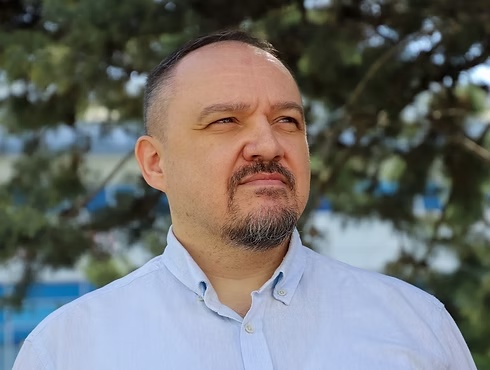
\includegraphics[width=4.5cm]{gorseller/yazar-oguz-ergin.jpg}}%
\hspace{0.7cm}%
\begin{minipage}[t]{10.5cm}%
\textbf{Prof.\ Dr.\ Oğuz Ergin}, bilgisayar mimarisi ve yüksek başarımlı işlemciler üzerine çalışan bir akademisyen, araştırmacı ve girişimcidir. Lisansını ODTÜ'de, yüksek lisans ve doktorasını New York'ta Binghamton Üniversitesi'nde tamamladı. Kariyerinin başında Intel'in Barselona araştırma merkezinde kıdemli araştırmacı olarak çalıştı; Türkiye'ye döndükten sonra TOBB ETÜ'de öğretim üyesi oldu, uzun yıllar bölüm başkanlığı ve üniversite yönetiminde danışmanlık görevleri yürüttü. 2024'ten bu yana Birleşik Arap Emirlikleri'nde Sharjah Üniversitesi Bilgisayar Mühendisliği Bölümü'nde profesör olarak görev yapmaktadır.%
\end{minipage}

\bigskip
\noindent
Araştırmaları; mikroişlemci mimarileri, bellek (özellikle DRAM) güvenliği ve güvenilirliği, enerji verimliliği, donanım hızlandırıcılar ve hata toleransı alanlarına odaklanır. Çalışmaları HPCA, MICRO ve ISCA gibi dünyadaki en saygın konferanslarda yayımlandı; 120'nin üzerinde uluslararası yayını ve çeşitli patentleri bulunmaktadır.

\medskip
\noindent
Akademi-sanayi köprüsünde aktif rol alan Ergin, Kasırga ve Yumruk şirketlerini kurarak savunma ve sivil alanlarda işlemci ve gömülü sistem çözümleri geliştirdi; Aselsan'a ve TUSAŞ'a danışmanlık yaptı ve Bilişim Vadisi'nde teknoloji danışma kurulunda görev aldı. ETH Zürih, Edinburgh ve Notre Dame üniversitelerinde misafir öğretim üyesi olarak bulundu.

\medskip
\noindent
Bugün, yetiştirdiği öğrenciler dünyanın önde gelen araştırma gruplarında ve teknoloji şirketlerinde görev alıyor; danışmanlığını yaptığı öğrenci ekipleri Teknofest yonga tasarımı yarışmalarında birçok derece elde etti. Oğuz Ergin, bilim ve teknoloji temelli yönetim anlayışını; liyakat, şeffaflık ve yüksek katma değerli üretim odaklı bir perspektifle toplumsal faydaya dönüştürmeyi amaçlıyor.


\end{document}
